\documentclass[a4paper,AutoFakeBold={2.7}]{ctexart} %纸张大小A4,文本类型为ctexart
%--------------------导言区:加载宏包,改变全局设置等--------------------%
\usepackage[colorlinks=true,urlcolor=black,linkcolor=black,citecolor=black]{hyperref}
%超链接宏包,消除外部网址链接,文内交叉引用链接,参考文献引用链接的方框,且将字色改为黑
\usepackage{amsmath}%数学宏包1
\usepackage{amssymb}%数学宏包2
\usepackage{bm}%公式加粗宏包
\usepackage{arydshln}%分块矩阵宏包
\usepackage{fontspec}%字体设置宏包
\usepackage{booktabs}%三线表宏包
\usepackage{array}%表格宏包
\usepackage{longtable}%跨页表格宏包
\usepackage{caption}%题注设置宏包
\usepackage{graphicx}%图片宏包
\usepackage{float}%浮动体宏包,强制让浮动体在Here位置
\usepackage{subfig}%子图宏包
\usepackage[left=2.5cm,right=2.5cm,top=2.5cm,bottom=2.5cm]{geometry}%页边距设置
\usepackage{wrapfig}%图片文字环绕宏包
\usepackage{listings}%代码高亮宏包
\usepackage{xcolor}%颜色处理宏包
\DeclareCaptionFont{heiti}{\heiti}%为caption宏包定义heiti命令
\captionsetup{labelsep=space,font={small,bf,heiti},skip=5pt}%题注设置
\setmainfont{Times New Roman}%英文设置为Times New Roman
\renewcommand{\baselinestretch}{1.25}%改变默认行距为1.25倍行距
\pagestyle{plain}%没有页眉,页脚包含页码
\ctexset{section={format={\heiti \zihao{-3} \bfseries}},
	subsection={format={\heiti \zihao{4} \bfseries},beforeskip=0pt,afterskip=0pt},
	subsubsection={format={\heiti \zihao{-4} \bfseries},beforeskip=0pt,afterskip=0pt}} %section样式设置

\lstset{
    language=Python,       % 设置语言为 Python
    basicstyle=\ttfamily,  % 基本样式
    keywordstyle=\color{blue},  % 关键字颜色
    commentstyle=\color{gray},  % 注释颜色
    stringstyle=\color{red},    % 字符串颜色
    numbers=left,        % 显示行号
    numberstyle=\tiny,   % 行号字体
    frame=single,        % 给代码加上边框
    breaklines=true      % 自动换行
    }
%---------------------------------------------------------------------%
\title{\heiti \zihao{-2} 《应用软件设计》课程设计 \\ \vspace{20pt} 数学试题库系统}%题目,黑体字,小二号大小
\author{陶宇行 \hspace{5pt} 226002262}
\date{2025/6/14}
%-----------------------------正文开始---------------------------------%
\begin{document}
\maketitle %标题

\begin{center}
	\addcontentsline{toc}{section}{摘要}%将摘要添加到目录中
	\section*{摘要}
\end{center}

使用vue3、TypeScript、Python Flask结合MySQL数据库开发了一个数学试题库系统。主要的界面有:登录注册页面,用户界面,管理员主要管理题目标签和题目,可以直接对数据库操作,故没有设计前端界面,但在设计数据库时,已经预留了用户身份,所以管理员前端界面可以随时拓展。在登录注册页面,用户(管理员)使用手机号和密码进行登录,注册时使用手机号码和手机短信验证码注册账号。

当用户忘记密码时,也可以通过手机号码和短信验证码来更换密码。在用户界面,用户可以查看所有的存储的题目信息,点击具体的题目,会跳转到对应的详细页面

\vspace{5pt}
\noindent \textbf{\heiti 关键词:}\songti 试题库系统,前后端分离开发,数据库

\newpage

\section{系统需求分析}

\subsection{需求概述}

Latex作为专业的数学排版工具受到广大用户的喜爱,通过Latex排版出的数学公式不仅美观优雅,更易于阅读。而网页作为内容传播最广泛的途径,通过网页建立一个数学试题库系统能够极大的方便数学内容的传播,但大多数题库在展示数学题目时,主要是以图片的形式展示,这样既不美观,也不清晰易读,通过KaTex库,我们能够将Latex排版的数学题嵌入到网页中并以正确的格式展示,相比于图片形式,显示效果优秀。并且在数据库中的存储形式也只是对应的Latex文本,节省了存储空间。

系统功能:

用户:查看题目、上传题目、查看个人信息、修改密码。

管理员:管理题目标签,管理题目。

\begin{figure}[H]
	\centering
	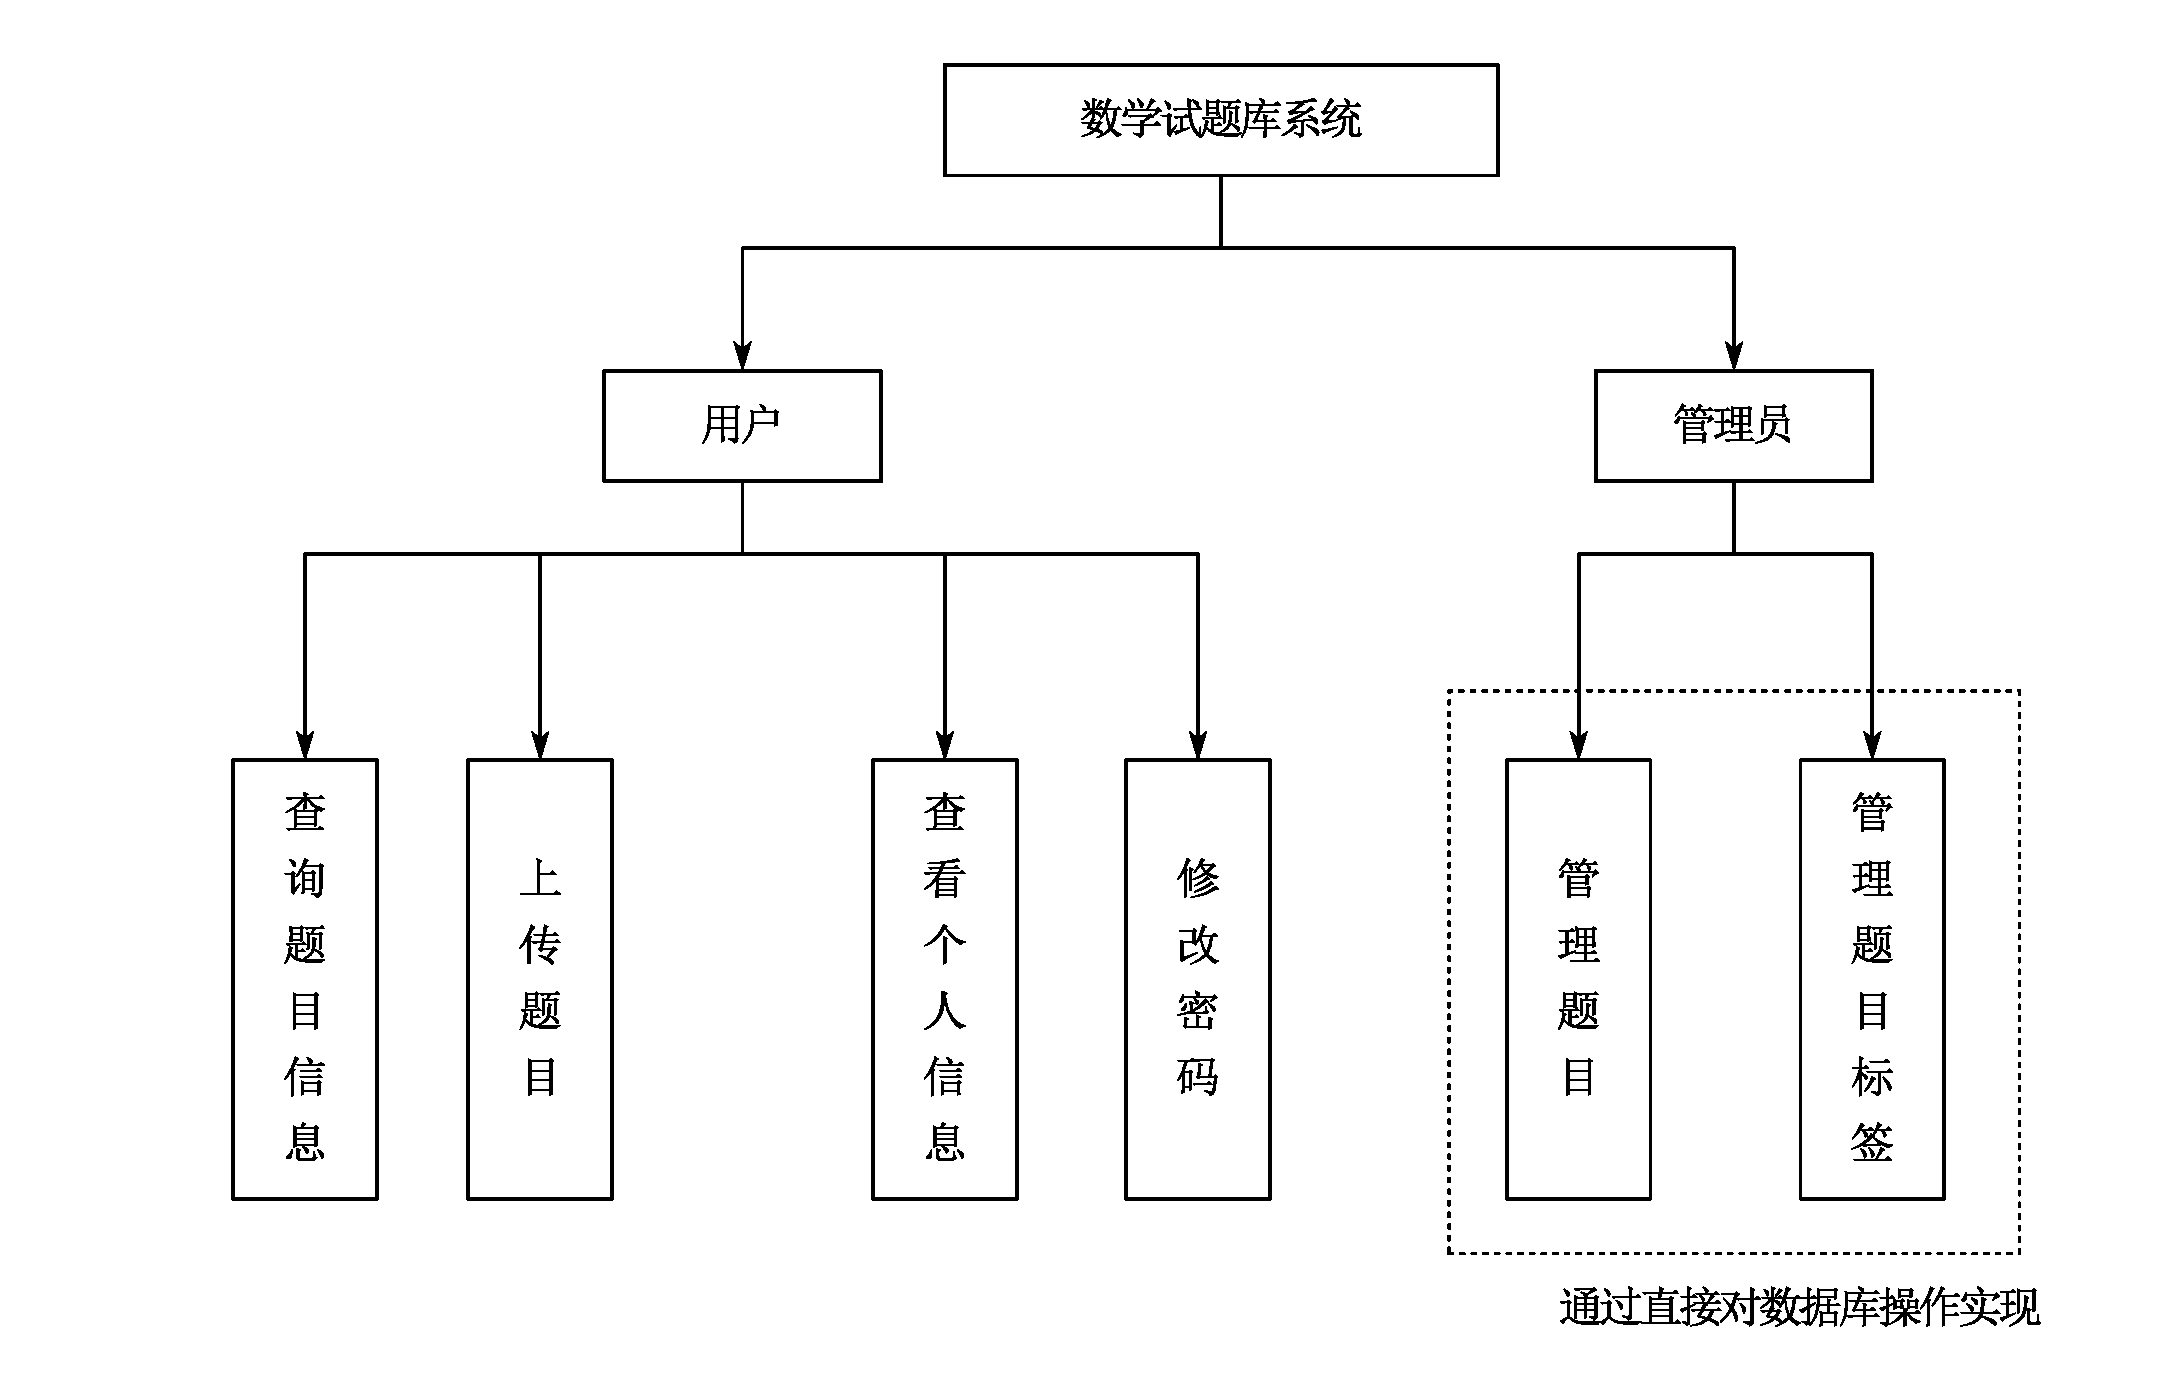
\includegraphics[width=\linewidth]{./图片/系统功能.pdf}
	\caption{系统功能}\label{系统功能}
\end{figure}

\subsection{用户工作流分析}

接下来对用户查看和上传题目的需求进行工作流分析,给用户展示的题目信息主要有两种形态:1、简略的题干;2、完整的题目内容。
当用户点击对应的题干后,会展示其完整内容,工作流程如下图所示:

\begin{figure}[H]
	\centering
	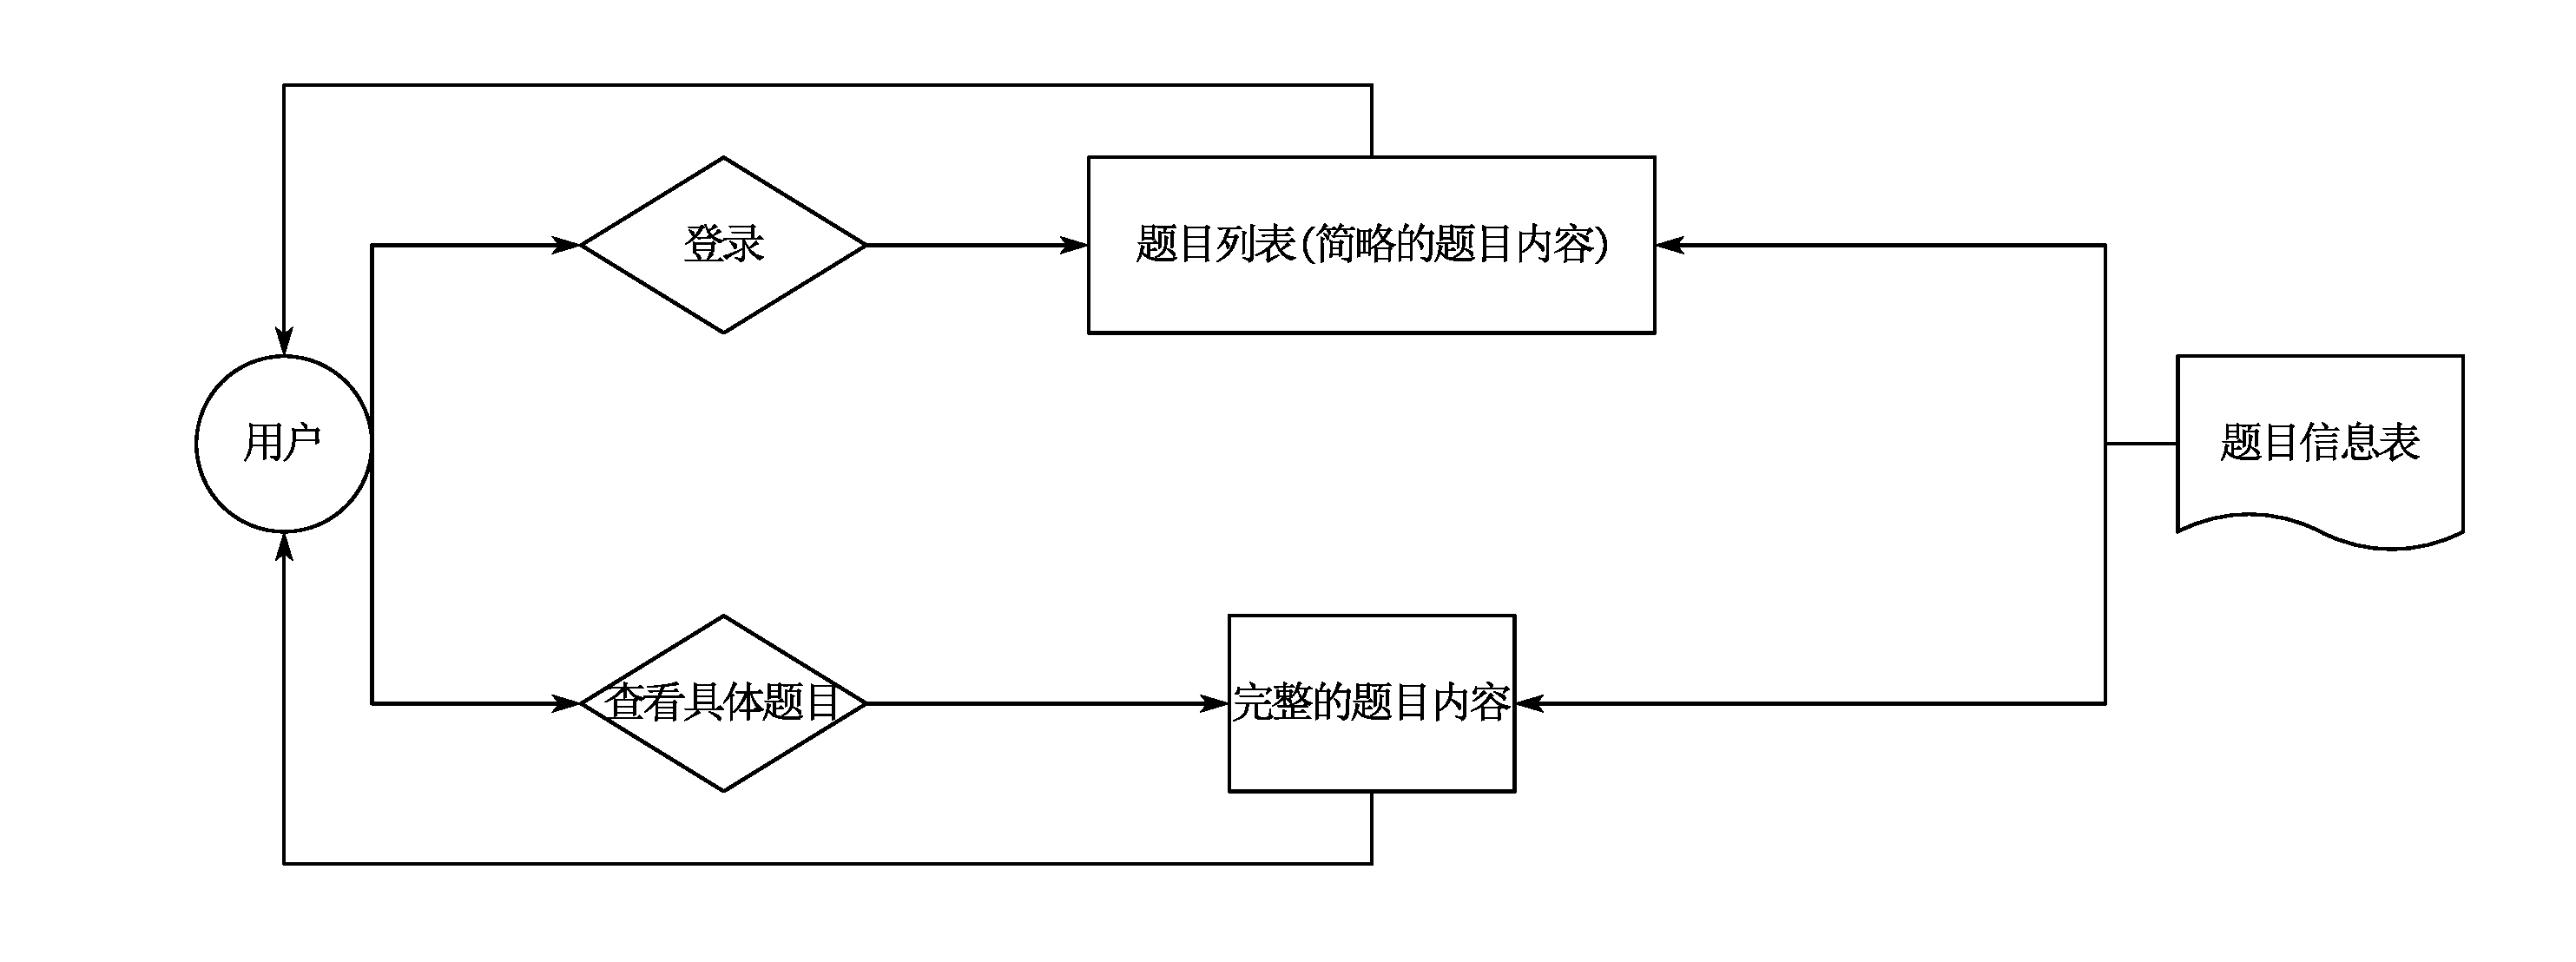
\includegraphics[width=\linewidth]{./图片/工作流程.pdf}
	\caption{工作流程}\label{工作流程}
\end{figure}

\section{开发框架选择}

1. 后端Python + Flask:选择 Python 作为后端开发语言,得益于其语法简洁、高效灵活以及丰富的第三方库生态,能够大幅提升功能实现和数据处理的效率。Flask 作为一个轻量级的 Web 框架,其简单易用的路由设计、灵活的扩展方式和较低的入门门槛,能够满足试题库系统在快速开发、调试和后期维护方面的需求。

2. 前端技术Vue 3 + TypeScript:前端部分选用了 Vue 3 框架,借助其组合式 API 能够更清晰地管理组件逻辑,实现高效复用和模块化开发。结合 TypeScript 的静态类型检查,进一步提高了代码的健壮性与可维护性,避免了运行时常见的错误,确保前端页面在交互性和动态显示方面的可靠性与流畅性。

3. 数据库MySQL:在数据存储方面,选用了成熟稳定的 MySQL 数据库。MySQL 以其卓越的性能、良好的事务支持和丰富的生态系统为系统提供可靠的数据管理后盾。对于数学试题库这种需要高效存储和快速查询的大规模数据场景,MySQL 能够提供稳定的性能保障,同时其广泛的社区支持和完善的文档也使得后续维护和优化更加便捷。

4. 数学公式渲染KaTeX:为了在网页上精准、迅速地展示 LaTeX 公式,我们采用了 KaTeX 渲染引擎。相较于其他渲染方案如 MathJax,KaTeX 拥有更高的展示速度和极强的兼容性,设计目标就是实现快速、轻量的公式渲染,因此在大量公式的实时显示中能显著降低加载延迟,能够在保证复杂数学公式准确显示的同时,有效降低页面加载压力,为用户提供流畅的数学体验。不过,为了追求效率,KaTeX 在支持 LaTeX 常用语法的同时放弃了部分高级扩展和定制化支持。但数学试题库系统主要需求是快速渲染大批量、标准数学公式,选用 KaTeX更好。

综合来看,该数学试题库系统采用 Python+Flask 构建后端服务,利用 Vue 3+TypeScript 构筑高度交互、类型安全的前端界面,并辅以 MySQL 数据库实现数据的高效存储与检索,最后通过 KaTeX 实现数学公式的高质量渲染。整体架构实现了前后端的高效分离,既满足当前业务需求,也为未来功能扩展和系统维护奠定了坚实基础。

\section{数据库设计}

主要设计了3张表:problems表,user表,tags表分别用于存储题目信息,用户信息,题目标签,其结构如下表所示:

\begin{table}[H]
	\caption{problems表}\label{problems表}
	\centering
	\begin{tabular}{p{3cm}<{\centering} p{3cm}<{\centering} p{3cm}<{\centering}}
		%p{3cm}规定列宽,\centering规定居中对其
		\toprule[1.5pt]
		字段&类型&说明\\
		\midrule[0.75pt]
		id&int&题目id\\
		content&varchar&题目内容\\
		tag&varchar&题目标签\\
		Uploader&varchar&上传者\\
		Upload\_time&datetime&上传时间\\
		\bottomrule[1pt]
	\end{tabular}
\end{table}

\begin{table}[H]
	\caption{tags表}\label{tags表}
	\centering
	\begin{tabular}{p{3cm}<{\centering} p{3cm}<{\centering} p{3cm}<{\centering}}
		%p{3cm}规定列宽,\centering规定居中对其
		\toprule[1.5pt]
		字段&类型&说明\\
		\midrule[0.75pt]
		id&int&标签id\\
		tag\_name&varchar&标签名\\
		\bottomrule[1pt]
	\end{tabular}
\end{table}

\begin{table}[H]
	\caption{user表}\label{user表}
	\centering
	\begin{tabular}{p{3cm}<{\centering} p{3cm}<{\centering} p{3cm}<{\centering}}
		%p{3cm}规定列宽,\centering规定居中对其
		\toprule[1.5pt]
		字段&类型&说明\\
		\midrule[0.75pt]
		id&int&用户id\\
		username&varchar&用户名\\
		telephone&varchar&电话\\
		password&varchar&密码\\
		role&varchar&身份(0表示用户,1表示管理员)\\
		\bottomrule[1pt]
	\end{tabular}
\end{table}

数据库结构E-R图如下所示:

\begin{figure}[]
    \centering
    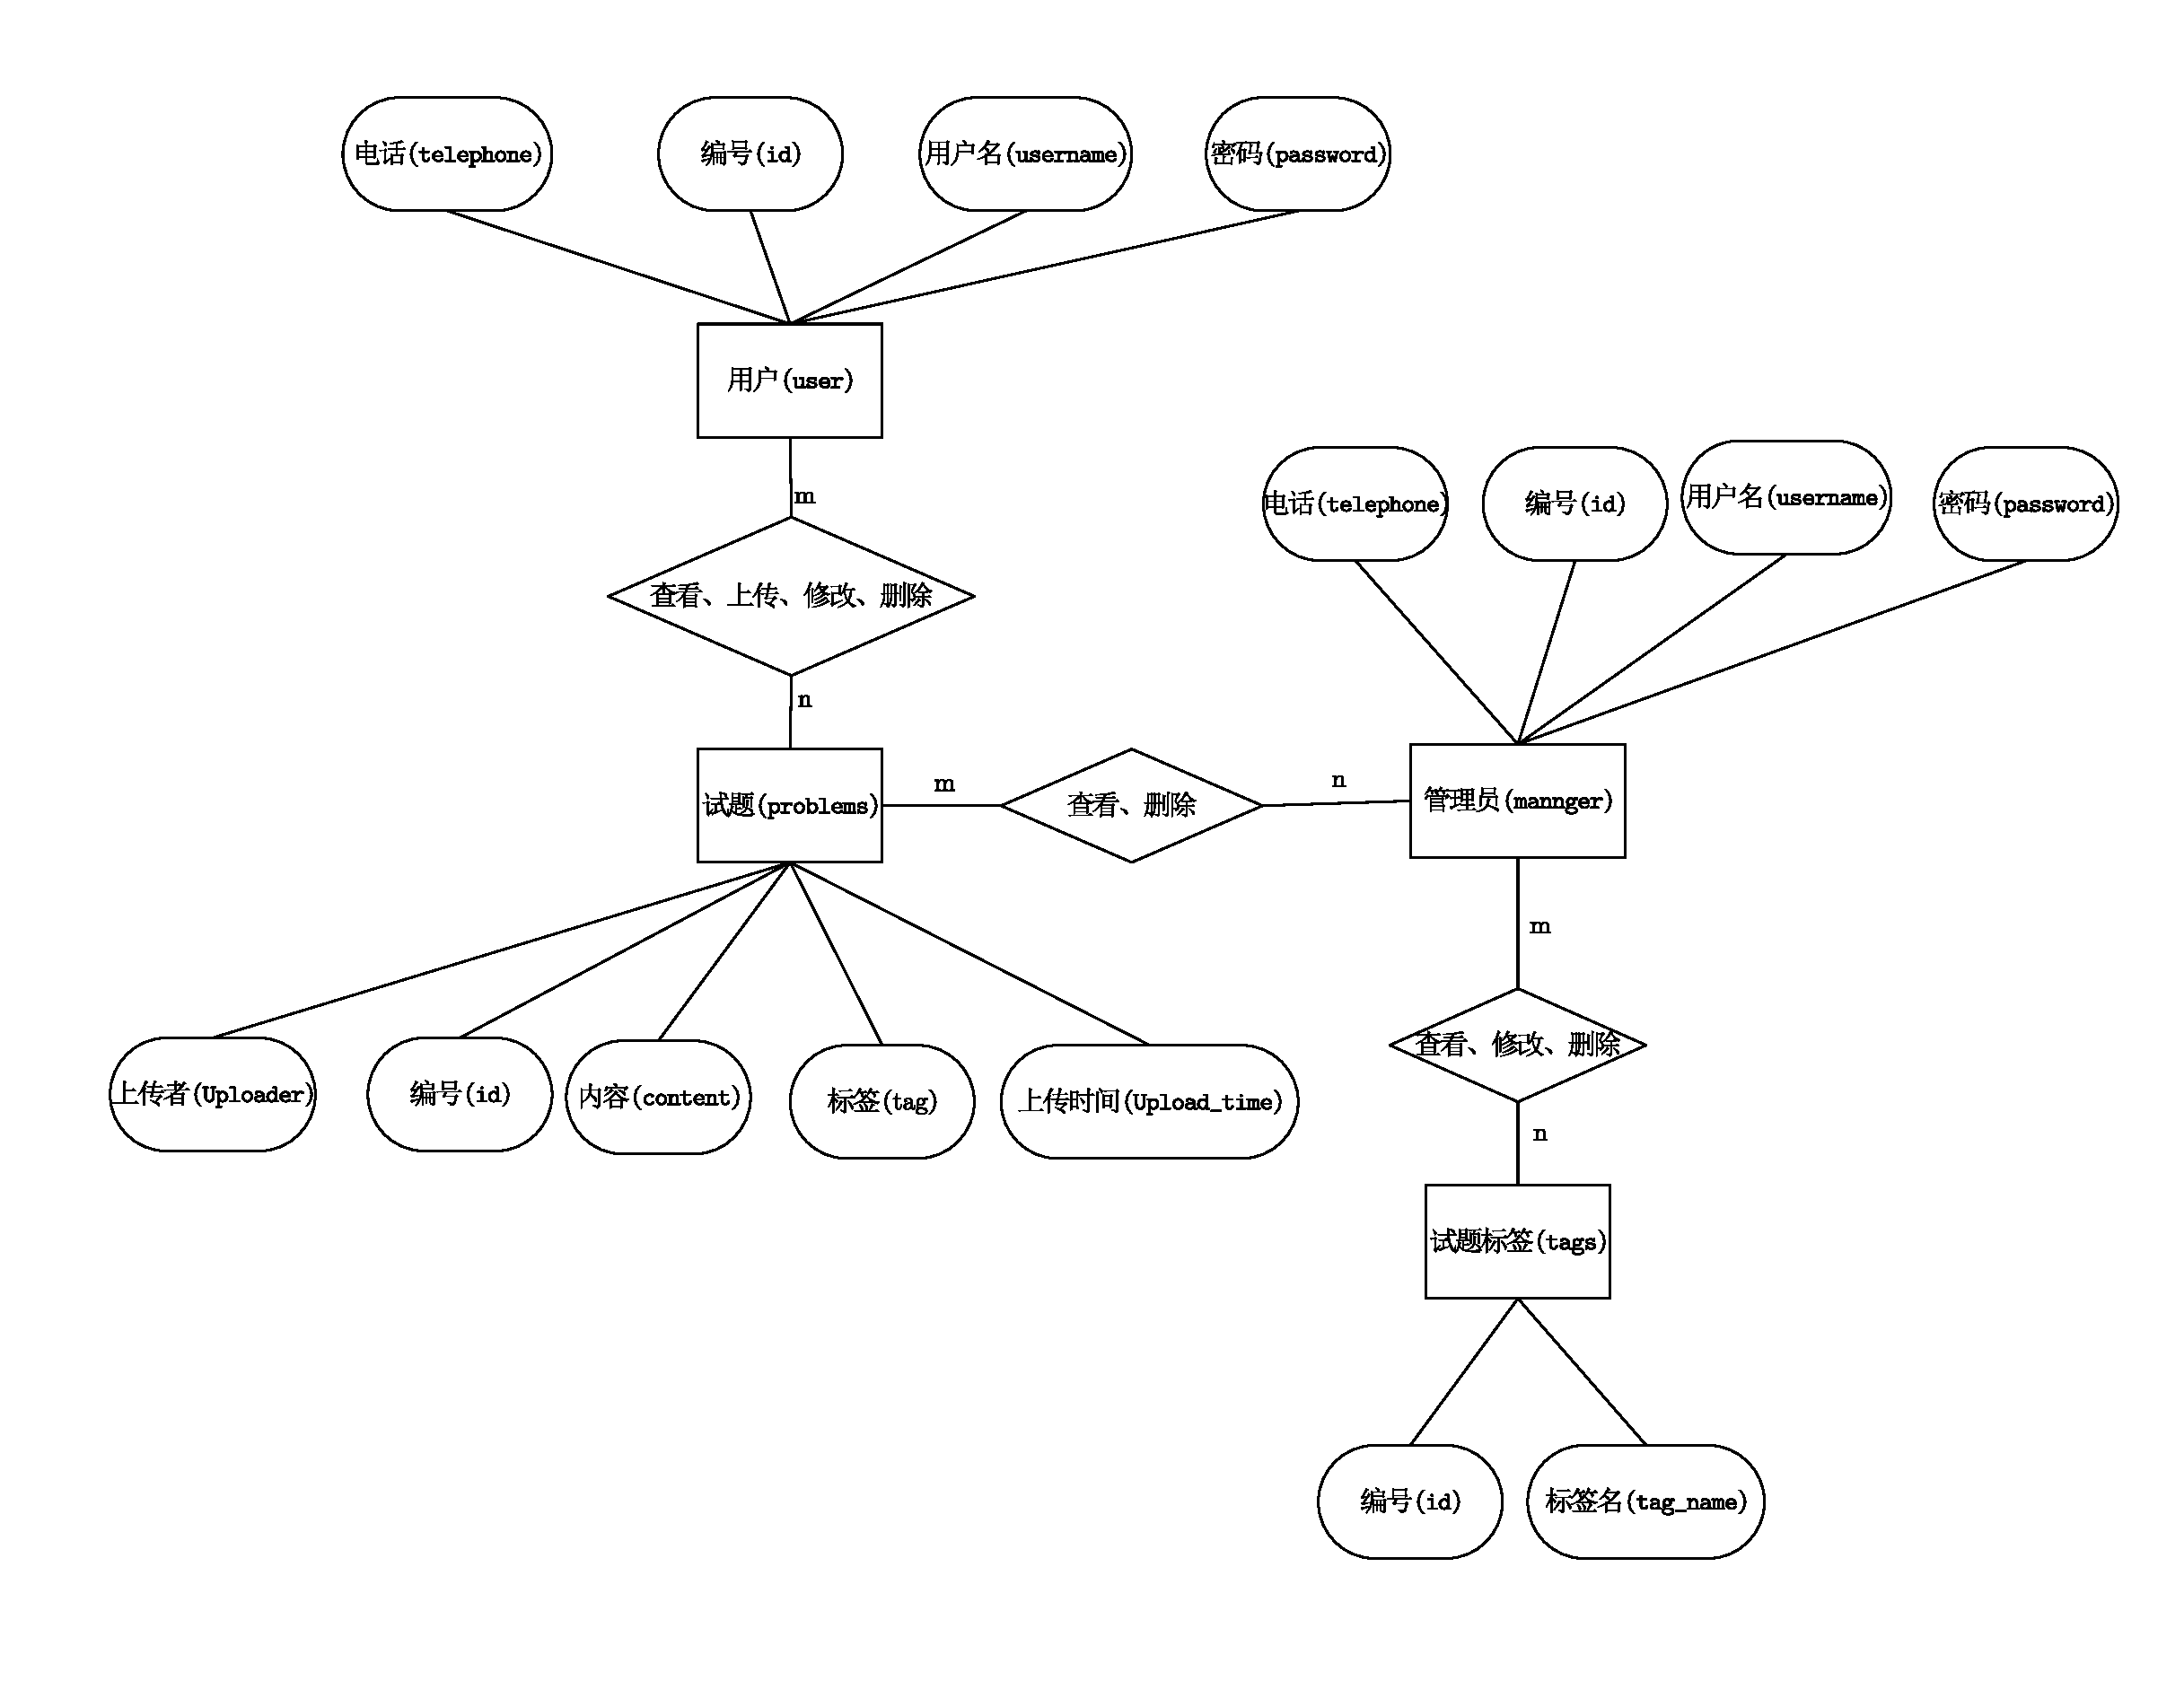
\includegraphics[width=0.7\linewidth]{./图片/数据库E-R图.pdf}
    \caption{数据库E-R图}\label{数据库E-R图}
\end{figure}

\section{后端设计}

使用Python + flask为系统提供后端支持。主要完成了下述功能:1、用户登录;2、用户注册(发送验证码的功能需要付费部署);3、获取用户信息;4、更改密码;5、获取所有题目;6、上传题目;7、获取所有标签。

\subsection{后端基本配置}

后端运行在127.0.0.1:5000上,而前端则运行在localhost:5173上,虽然127.0.0.1和localhost都是指本地主机地址,但为了防止出现跨域报错,还是直接配置后端允许所有来源访问比较好,配置的代码如下:
\begin{lstlisting}
CORS(app, resources={r"/*": {"origins": "*"}})
\end{lstlisting}

在后端代码中还定义了两个工具函数:\verb|get_token_phone|和\verb|get_token_user|,分别用于从token中获取电话和用户名信息。

最后,定义了两个类:Problem类和Tag类,它们的成员变量与数据库中的表结构一一对应,定义这两个类是为了方便上传题目和上传新标签(通过直接对数据库操作实现,但仍然保留以便随时拓展)两个方法的执行。定义这两个类的代码如下所示:

\begin{lstlisting}
class Problem(db.Model):
    __tablename__ = 'problems'
    id = db.Column(db.Integer, primary_key=True)
    content = db.Column(db.String, nullable=False)
    tag = db.Column(db.String, nullable=False)
    Uploader = db.Column(db.String, nullable=False)
    Upload_time = db.Column(db.DateTime, nullable=False)


class Tag(db.Model):
    __tablename__ = 'tags'
    id = db.Column(db.Integer, primary_key=True)
    tag_name = db.Column(db.String, nullable=False, unique=True)
\end{lstlisting}

\subsection{后端接口逻辑}

1、用户登录方法\verb|user_login|:请求方式为POST,先从前端获取到用户输入的电话号码和密码信息,将获取到的信息加入到sql查询语句中,作为条件查询where的条件,如果查询到的数据非空,则说明输入的电话号码和密码正确,那就返回登录成功的信息并生成token一并返回。否则,输入的电话号码或者密码与数据库中的记录不匹配,则返回用户名或密码错误的信息。

2、获取用户信息方法\verb|usermsg|:请求方式为GET,首先从请求头中提取token,然后调用工具函数\verb|get_token_phone|获取当前用户电话号码,将获取到的电话号码加入到sql查询中,从数据库中查询电话号码对应的用户信息。若成功查询到记录,则返回查询到的数据,否则返回查询失败的消息。

3. 修改密码方法:\texttt{user\_pwd\_change}:请求方式为 POST,使用异常处理机制包裹所有的执行逻辑,防止数据库错误或 token 解码出错时直接崩溃。一旦报错,使用 \texttt{rollback()} 撤销数据库未提交的修改,避免脏数据。具体的执行逻辑为:先从前端请求体 JSON 中获取旧密码 \texttt{old\_pwd} 和新密码 \texttt{new\_pwd},再从请求头中获取 token,用于身份校验。如果前端未传 token,直接返回 400 Bad Request。若成功获取到 token,则使用工具函数 \texttt{get\_token\_phone} 获取当前用户电话号码。电话号码和旧密码将作为查询条件,然后使用原生 SQL 检查手机号 + 原始密码是否存在于数据库。采用参数化查询的方式以防止 SQL 注入。如果查询到的数据为空,则说明原密码错误,返回错误信息。若数据不为空,则通过 update 语句更新数据库中的对应记录,完成密码更新。

4、获取所有题目方法\texttt{get\_problems}:请求方式为GET,同样使用异常处理机制\texttt{try-except}机制包裹整个执行逻辑,防止执行 SQL 时出错导致程序崩溃,同时若发生异常,则返回具体的异常信息,方便调试。具体的执行逻辑为:从数据库problems表中查询所有的题目记录,遍历 查询结果,每一条记录是一个元组。构造python字典,使得每条题目的信息结构化。最后返回json格式的数据。

5、上传题目方法\texttt{add\_problem}:请求方式为POST。首先通过 \texttt{request.get\_json()} 获取请求体中的数据,如果没有数据则返回 400 错误。接着从数据中提取题目内容 content(必填)、标签 tag(默认为“无标签”)、上传人 Uploader(默认“anonymous”,但实际使用的是从 token 中解析的用户名)以及上传时间字符串 Upload\_time。对 content 和 Upload\_time 进行非空校验,如果缺失则返回 400 错误。上传时间字符串采用 ISO 格式,通过 \texttt{datetime.datetime.fromisoformat()} 解析为 datetime 对象,解析失败会返回格式错误的 400 响应。然后查询数据库 problems 表当前最大 id,以便手动分配新题目的唯一 ID。通过请求头中的 token,调用工具函数 \texttt{get\_token\_username()} 获取当前登录用户的用户名,确保上传人信息的准确性。构造新的 ORM 对象 Problem(通过自定义的Problem类),包含新生成的 ID、题目内容、标签、上传者用户名和上传时间。将该对象添加到数据库会话并提交事务,若数据库操作失败则回滚并返回错误。最终返回新题目的 ID 表示上传成功。题目内容中的 LaTeX 代码作为普通字符串直接存储,后续由前端或渲染程序负责正确解析和显示,保证了 LaTeX 代码的原样保存和灵活使用。

6、获取所有标签方法\texttt{get\_tags}:请求方式为GET,通过执行一条 SQL 语句 SELECT id, tag\_name FROM tags,获取标签表中所有标签的 ID 和名称。查询结果使用 fetchall() 方法获取所有记录,并将每条记录封装成字典格式,包含 id 和 tag\_name 两个字段,最终组成一个标签列表。接口成功执行时返回包含标签列表的 JSON 数据。若在查询过程中出现异常,接口会捕获异常并返回错误信息。

\section{前端设计}

使用 vue3 + TypeScript,还有Element Plus UI库设计前端界面。前端代码的目录结构如下所示:

\begin{figure}[H]
	\centering
	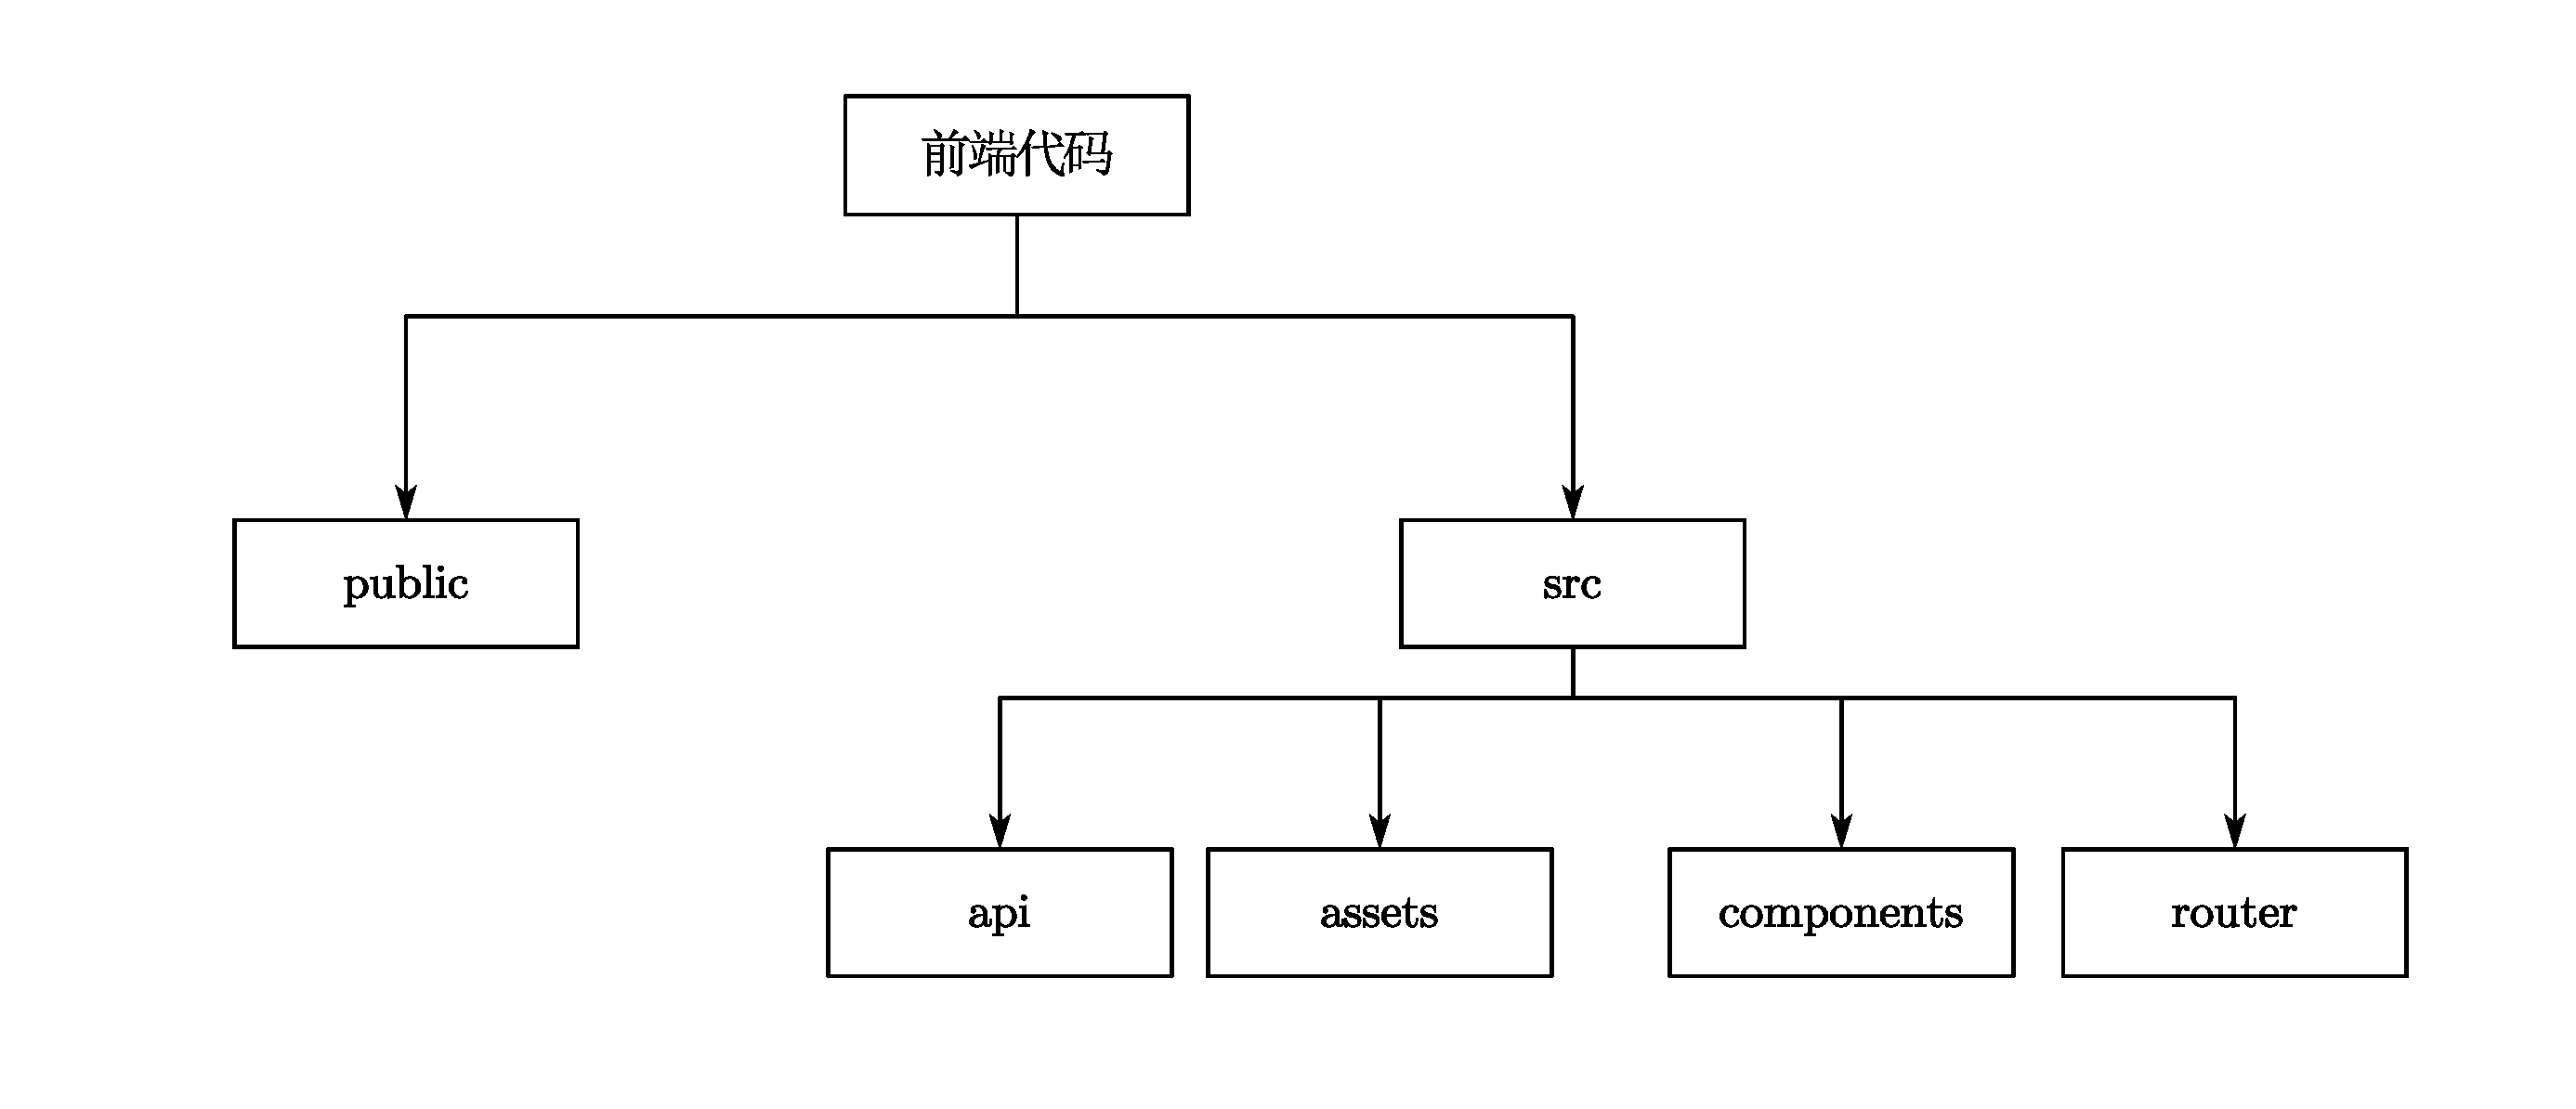
\includegraphics[width=\linewidth]{./图片/目录结构.pdf}
	\caption{目录结构}\label{目录结构}
\end{figure}

\subsection{目录功能说明}
主要说明src目录下的几个文件夹的作用:

1、api目录下的index.ts文件为项目提供统一的 HTTP 请求工具,并在请求发送前自动附加 token 到请求头。

2、assets目录存放了图片用于样式设计。

3、components目录存放vue组件。

4、router目录下的index.ts文件存放了vue router核心配置文件,用于管理页面路由,设置默认路径跳转。

\subsection{api目录下index.ts文件详细说明}

\verb|api\index.ts|文件源码如下:

\begin{lstlisting}
import axios from "axios";
import type {AxiosInstance, InternalAxiosRequestConfig} from "axios";

const http: AxiosInstance = axios.create({
    baseURL: "http://127.0.0.1:5000",
    timeout: 5000,
});

http.interceptors.request.use(
    (config: InternalAxiosRequestConfig) => {
        const token = localStorage.getItem("token");
        if (token) {
            if (!config.headers) {
                (config.headers as any) = {};
            }
            (config.headers as any)["token"] = token;
        }
        return config;
    },
    (error) => Promise.reject(error)
);

export default http;
\end{lstlisting}

这里首先导入了axios主库、Axios 实例的类型定义:AxiosInstance还有Axios请求配置的内部类型:InternalAxiosRequestConfig(包含请求头、参数等,比外部暴露的 AxiosRequestConfig 更全面)

然后创建了一个名为http的Axios实例,设置将所有请求将默认加上baseURL属性所定义的前缀,请求超时时间设置为 5000 毫秒。

接下来设置请求拦截器,用于在发送请求前进行统一处理,主要逻辑如下:

1、token注入:使用localStorage.getItem("token")获取本地存储的登录令牌。如果有 token,则确保 config.headers 存在。如果不存在则手动赋空对象(使用 as any 避开类型限制)。使用是对象赋值语法config.headers["token"] = token把 token 添加到请求头中

2、错误处理:第二个函数参数用于处理拦截器执行失败的情况,直接将错误返回 Promise.reject。

最后导出配置好的axios实例,以便其他代码文件使用统一配置的带 token 的请求。
\subsection{router目录下index.ts文件详细说明}

\verb|router\index.ts|文件源码如下:

\begin{lstlisting}
// src/router/index.ts
import { createRouter, createWebHistory } from "vue-router";
import type { RouteRecordRaw } from "vue-router";
const LogRes = () => import("../components/LoginRegister.vue");
const user = () => import("../components/MainWindow.vue");

const routes: RouteRecordRaw[] = [
  {
    path: "/",
    redirect: "/login",
  },
  {
    path: "/login",
    component: LogRes,
    meta: {
      title: "登录",
    },
  },
  {
    path: "/user",
    component: user,
    meta: {
      title: "用户界面",
    },
  },
];

const router = createRouter({
  history: createWebHistory(),
  routes,
});

export default router;

\end{lstlisting}

首先导入必要的模块:createRouter, createWebHistory,RouteRecordRaw。createRouter是一个创建路由实例的方法,createWebHistory表示使用 HTML5 的 History 模式(即路径形式如 /login,而不是 hash 模式的 \#/login)。RouteRecordRaw: 是 Vue Router 中定义路由记录的类型。

然后使用动态 import() 的方式懒加载组件,也就是“用到才加载”,可以减小首屏体积,提高性能。其中:LogRes 是登录注册页组件,user 是用户主界面组件。

随后定义路由规则,在列表routes中,每个元素是一个对象,每个对象都是一条路由规则。路由规则中:path表示 URL 路径;component:表示对应要加载的组件;meta为自定义数据,这里用于设置标题;redirect表示重定向路径

在路由规则中,最主要的操作是将访问根路径/时的地址自动重定向到 /login。防止打开前端界面时,由于访问的是根目录而出现的not found错误,这样就不必在地址栏手动加上/login地址,优化了使用体验。

最后将定义好的路由规则导出,供main.ts文件使用。

将上述axios配置和router配置好后,在程序的主入口main.ts中使用,main.ts文件代码如下:

\begin{lstlisting}
import { createApp } from 'vue'
import App from './App.vue'
// Element Plus
import ElementPlus from 'element-plus'
import 'element-plus/dist/index.css'
import router from './router'
// 引入 axios 配置
import http from './api'
const app = createApp(App)
// 使用 Element Plus 插件
app.use(ElementPlus)
// 使用路由
app.use(router)
// 将 axios 挂载到全局
app.config.globalProperties.$axios = http
// 挂载到 #app
app.mount('#app')
\end{lstlisting}

\subsection{vue组件详细说明}

一共有7个vue组件:1、ChangePassword.vue;2、IndividualMessage.vue;3、LatexRender.vue;4、LoginRegister.vue;5、MainWindow.vue;6、QuestionViewer.vue;7、UploadProblems.vue。

ChangePassword.vue组件中定义了changePassword()方法,将请求发送给后端user\_pwd\_change()方法进行处理。

IndividualMessage.vue组件实现了获取个人信息getData()方法,前端请求由后端usermsg()方法处理。

LatexRender.vue是一个工具组件,用于控制网页上公式的渲染,并不显示实际的页面,主要被QuestionViewer.vue组件引用。

QuestionViewer.vue组件控制题目的两种显示方式:1、简略显示题干;2、完整的显示题目详情。为了方便题目的显示和查看,实现了筛选和分页功能,其中筛选功能分为按题目标签筛选和按上传时间筛选,获取题目的功能由fetchProblems()方法完成,组件中获取题目的请求交由后端get\_problems()方法处理。

LoginRegister.vue组件用于用户的登录和注册以及找回密码功能,由于注册和找回密码功能发送手机验证码的功能需要付费部署,所以这两个功能的代码暂时以注释的形式存在。用户登录的前端请求由login()方法发送给后端,交由后端user\_login()方法处理。

UploadProblems.vue组件控制题目的上传,用户可在输入框中输入Latex语句,在输入框下方会显示Latex语句的实时预览效果。通过uploadProblem()方法发送上传请求,上传题目的请求由后端add\_problem()方法处理。

MainWindow.vue组件是用户登录后系统的主要界面,整合了QuestionViewer.vue、IndividualMessage.vue、ChangePassword.vue、UploadProblems.vue。通过页面左侧的导航栏,控制以上四个组件的显示。

总体结构如下图所示:

\begin{figure}[H]
	\centering
	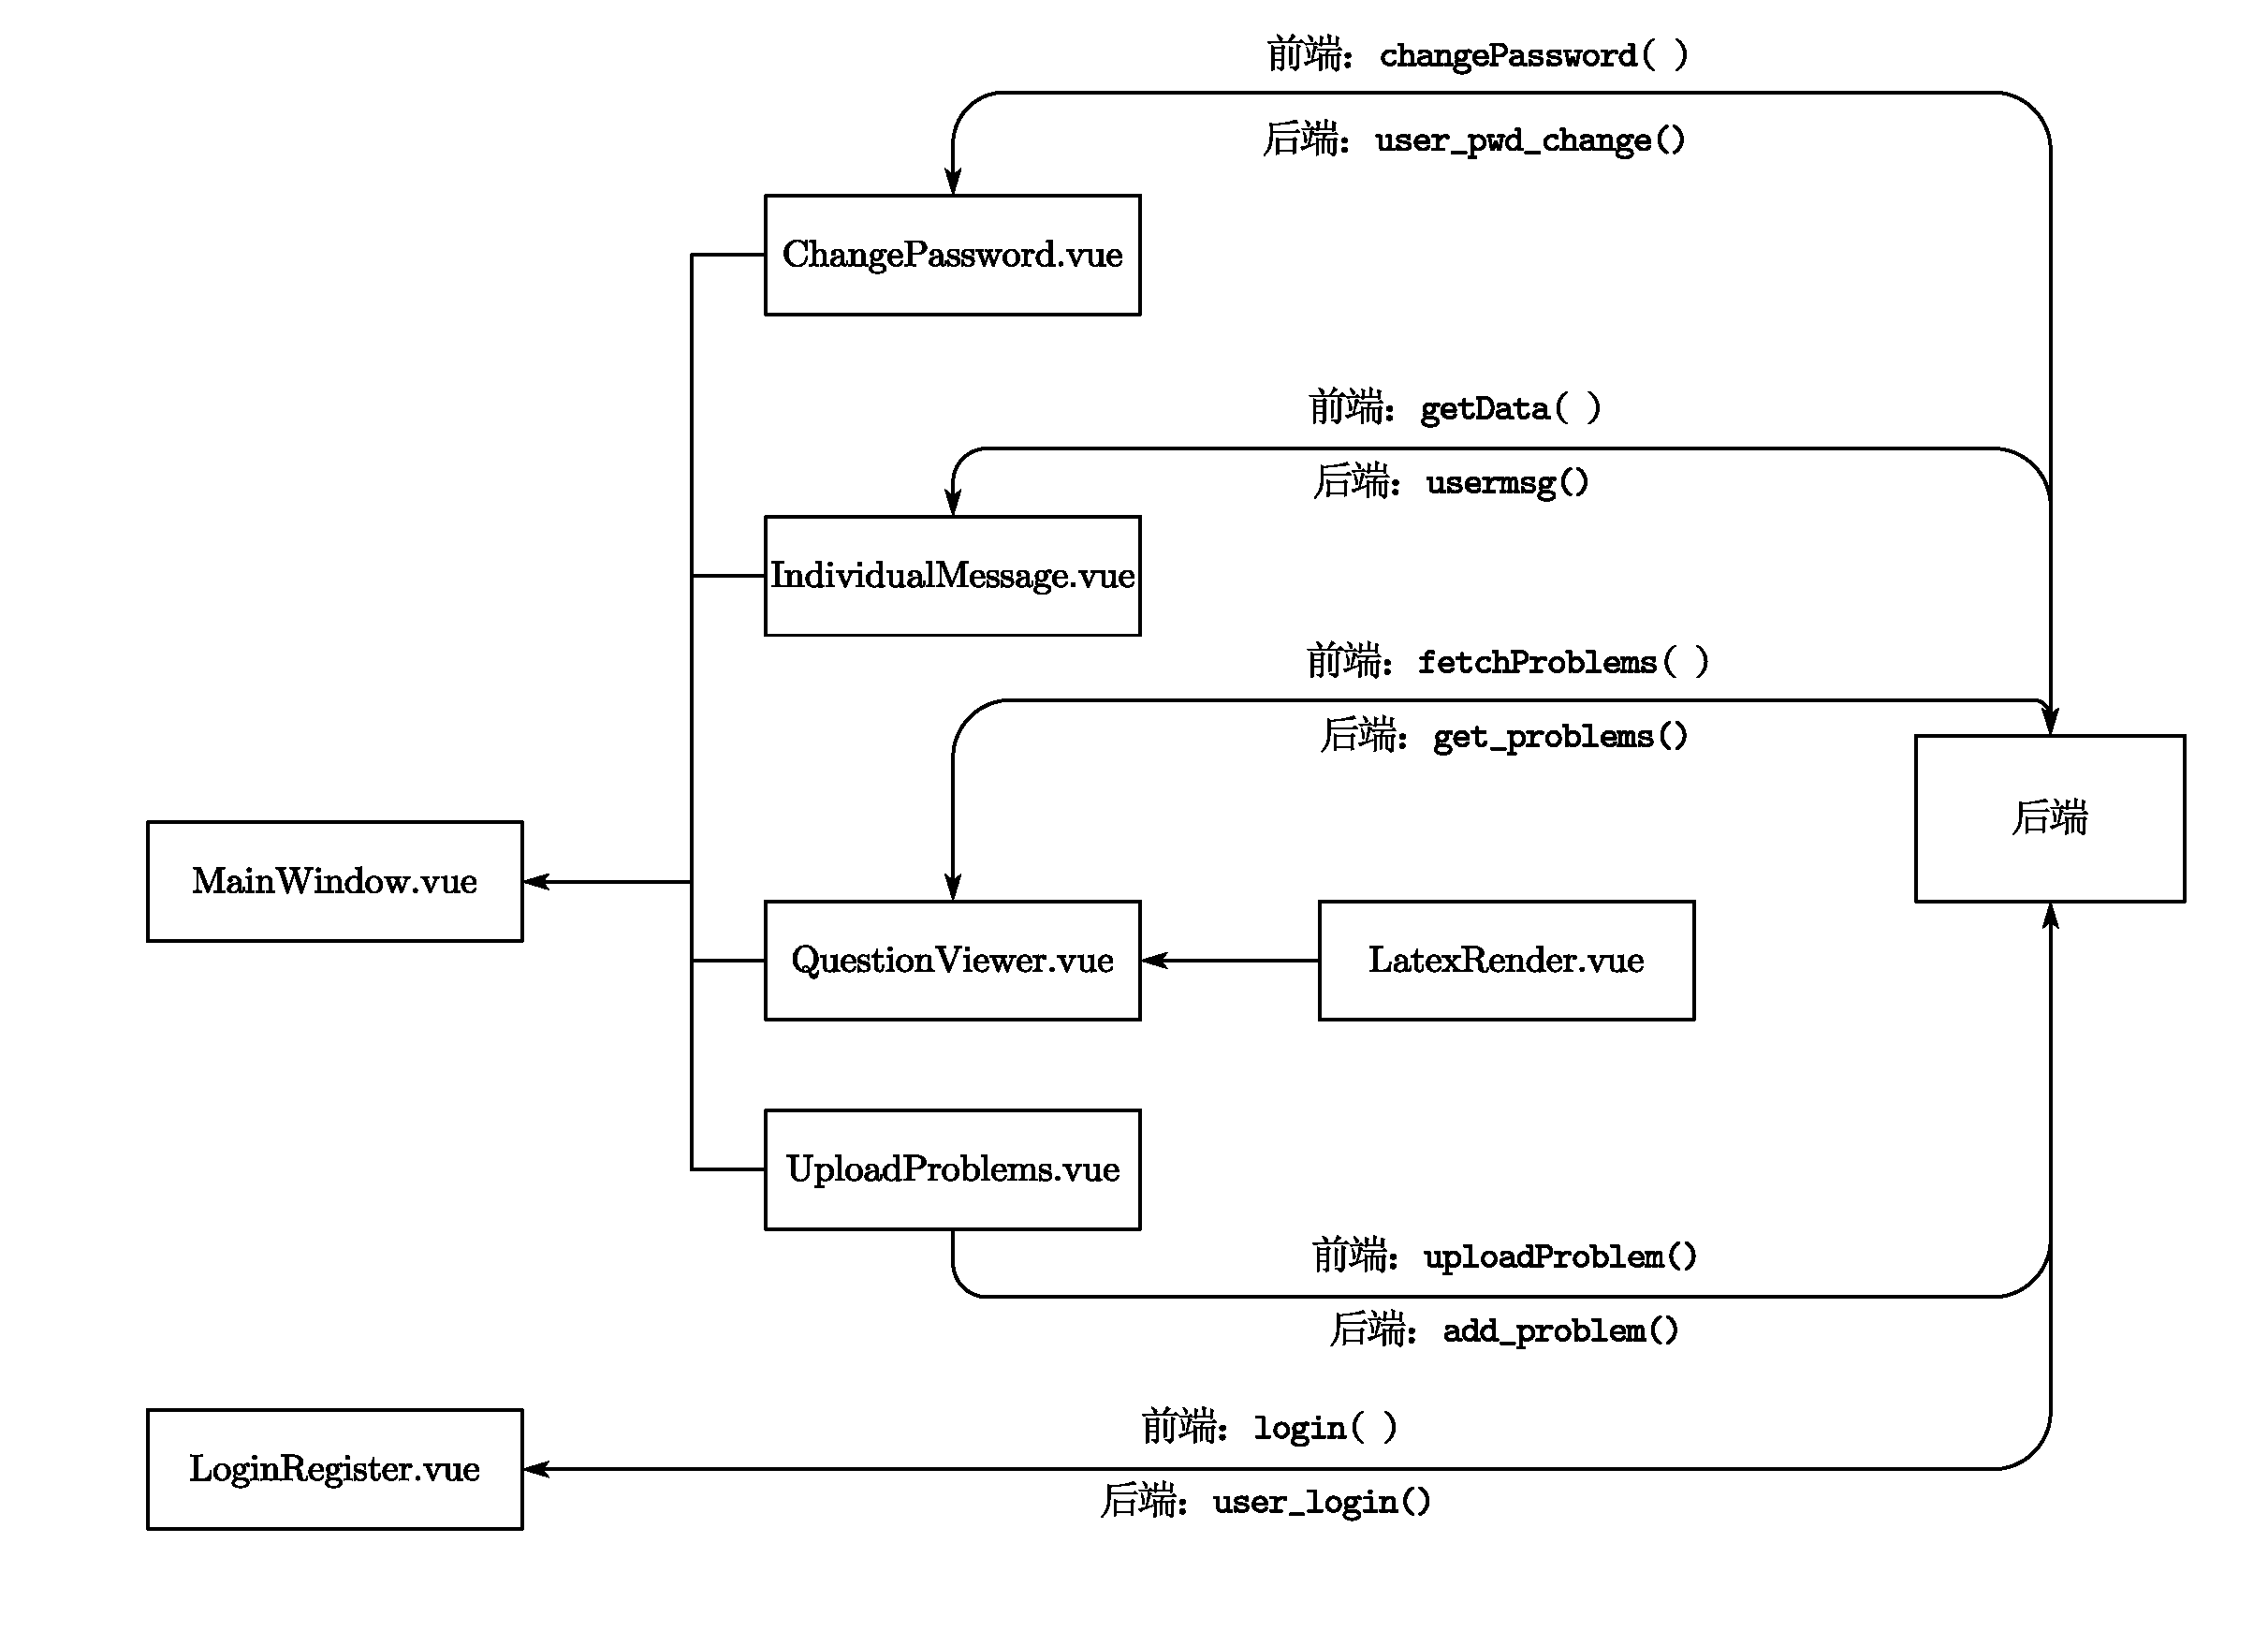
\includegraphics[width=0.85\linewidth]{./图片/前端结构.pdf}
	\caption{前端结构}\label{前端结构}
\end{figure}

\subsection{系统体验优化}

\subsubsection{手机号格式验证}

为了防止在登录或者注册或者忘记密码时输入不正确格式的手机号,在向后端发起请求前,就对手机号的格式进行验证,验证的方法如下:

\begin{lstlisting}
const checkMobile = (_rule: any, value: string, callback: (error?: Error) => void) => {
    const regMobile = /^(0|86|17951)?(13[0-9]|15[0-35-9]|17[0-8]|18[0-9]|14[5-7]|19[0-9])[0-9]{8}$/;
    if (regMobile.test(value)) {
        callback();
    } else {
        callback(new Error('手机号码格式不正确'));
    }
};
\end{lstlisting}

通过正则表达式的方法进行匹配,检测方法中,正则表达式部分含义是:从字符串的第一个字符开始匹配到字符串的最后一个字符结束。(0|86|17951)?的作用是匹配可选的国家/地区码前缀其中:0表示某些老格式;86表示中国大陆的国家区号;17951是一种拨号方式的前缀(如 IP 电话)。?表示表示这部分可以没有,即是否有区号是可选的。(13[0-9]|15[0-35-9]|17[0-8]|18[0-9]|14[5-7]|19[0-9])则是用于手机号前3位段号的校验。[0-9]{8}表示紧跟着的 8 个数字,构成手机号的后 8 位。综合起来,构成了电话号码的正则匹配,过滤掉无效的电话号码格式。

\subsubsection{密码输入框自动清空}

用户在修改密码时,如果输入的原密码错误,仅仅只是弹出原密码错误的消息,但并不会清空密码框,导致用户想要重新输入时需要手动清空密码输入框,操作变得十分麻烦,同时,即使密码修改成功,密码输入框也不会清空,而是留有修改时的输入记录。因此,需要在修改密码的方法中加入清空输入框的相关操作,优化后的修改密码方法代码如下:

\begin{lstlisting}
const changePassword = () => {
if (!formRef.value) return;
formRef.value.validate((valid) => {
    if (!valid) return;
    // 检查新密码与确认密码
    if (form.value.check_pwd !== form.value.new_pwd) {
        ElMessage.error("新密码与确认密码不一致");
        // 清空表单数据
        form.value.old_pwd = "";
        form.value.new_pwd = "";
        form.value.check_pwd = "";
        return;
    }
    // 从本地存储中获取 token
    const token = localStorage.getItem('token');
    if (!token) {
        ElMessage.error("登录已过期,请重新登录");
        return;
    }
    // 将请求数据和 token 一同提交
    axios
            .post("http://127.0.0.1:5000/user/pwd_chg", form.value, {
                headers: {
                    token: token,
                },
            })
            .then((res) => {
                if (res.data.status === 200) {
                    ElMessage.success(res.data.msg);
                } else {
                    ElMessage.error(res.data.msg);
                }
            })
            .catch((error) => {
                console.error("修改密码失败:", error);
                ElMessage.error("修改密码失败,请重试");
            })
            .finally(() => {
                // 清空表单数据
                form.value.old_pwd = "";
                form.value.new_pwd = "";
                form.value.check_pwd = "";
            });
});
};
\end{lstlisting}

通过添加\verb|form.value.old_pwd = ""|、\verb|form.value.new_pwd = ""|、\verb|form.value.check_pwd = ""|三个操作,实现消息弹出后清空输入框的功能。

\subsubsection{上传题目后页面自动刷新}

用户上传完题目时,页面不会自动刷新,导致新上传的题目不会立即显示,而是需要手动刷新后才会出现新上传的题目,为了解决这一问题,采用事件监听机制以实现自动刷新的功能。

首先对用户上传题目时的工作流进行分析:用户通过UploadProblems.vue组件编辑题目,调用其中的uploadProblem()方法实现上传题目到后端的操作,最后前端页面刷新后即可显示出新的题目。因此,要在题目上传成功时,发射题目上传成功的事件。题目的浏览是通过QuestionViewer.vue组件实现,所以要在这个组件中定义刷新页面的方法,而QuestionViewer.vue组件中已经定义好了获取所有题目的方法fetchProblems(),那么刷新页面的方法就可以是它。又由于UploadProblems.vue组件和QuestionViewer.vue组件都是主窗口MainWindow.vue组件的子组件,因此UploadProblems.vue组件的信号要发射到MainWindow.vue组件上,并且QuestionViewer.vue组件中定义的刷新方法要暴露给MainWindow.vue组件使用,从而在MainWindow.vue组件中定义处理时间的槽函数,这样就可以实现自动刷新功能。

总的流程如下图所示:

\begin{figure}[H]
    \centering
	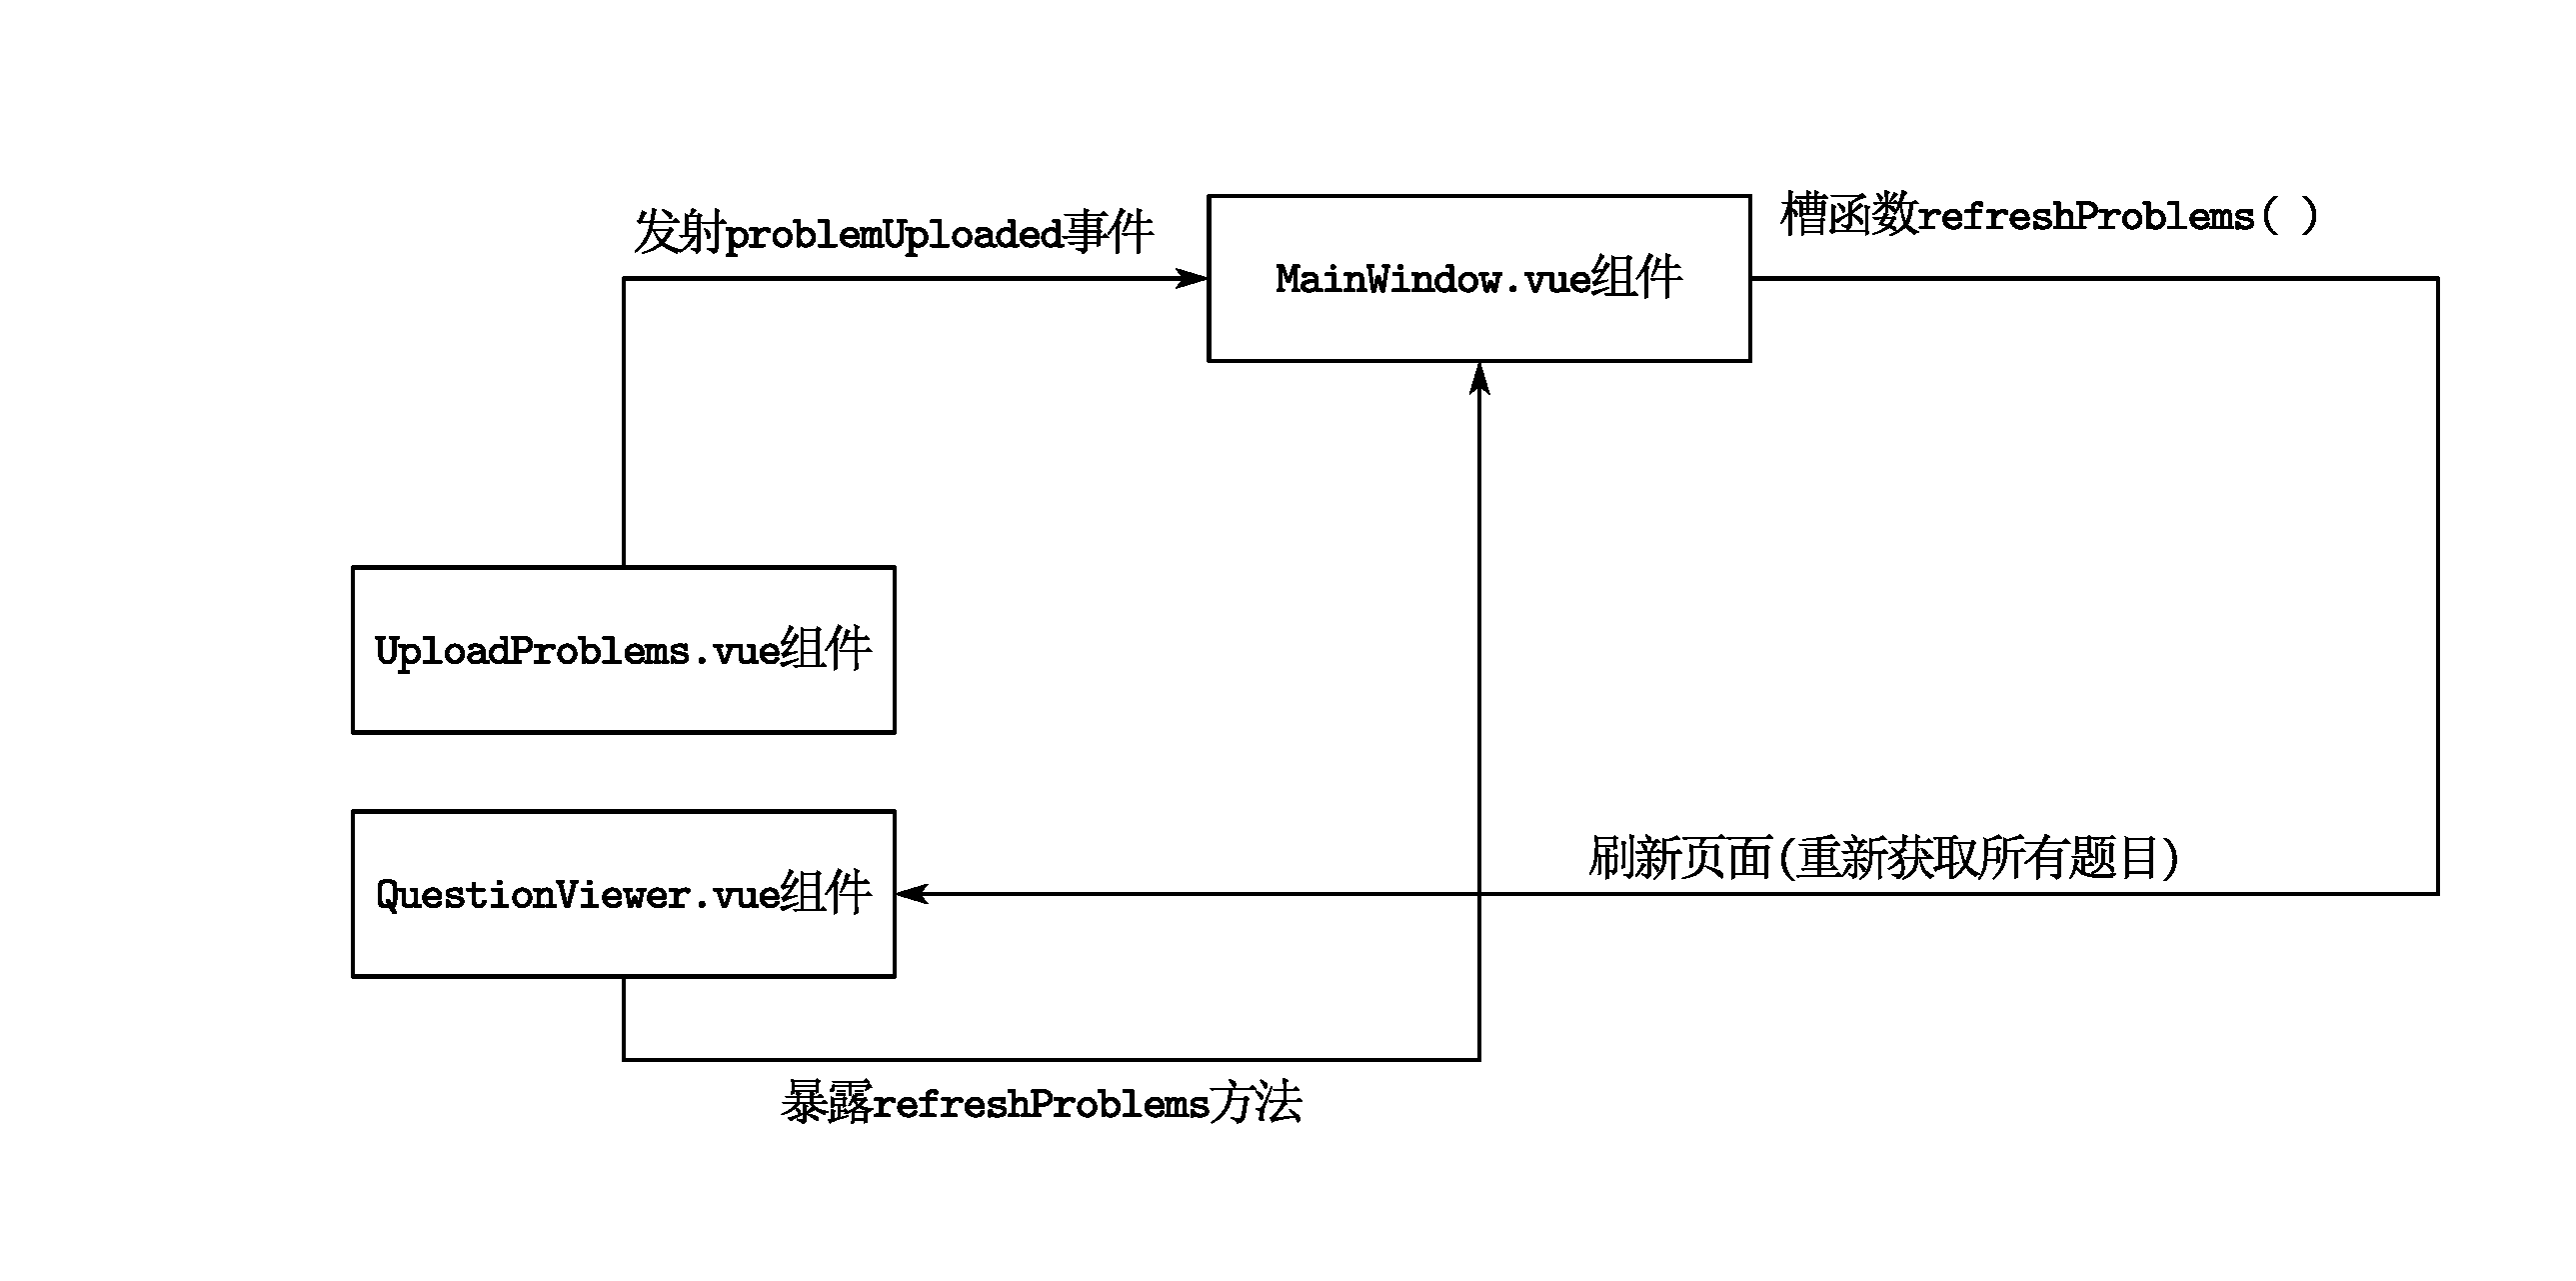
\includegraphics[width=0.7\linewidth]{./图片/自动刷新方法.pdf}
	\caption{自动刷新方法}\label{自动刷新方法}
\end{figure}

代码中实现方式如下:

UploadProblems.vue组件发射problemUploaded事件:

\begin{lstlisting}
const emit = defineEmits(['problemUploaded']) //定义发射事件

// 上传题目到后端
async function uploadProblem() {
    if (!latexContent.value.trim()) {
        alert("请输入 LaTeX 语句");
        return;
    }
    if (!selectedTag.value) {
        alert("请选择题目标签");
        return;
    }

    // 从 localStorage 中取出 token 和用户名
    const token = localStorage.getItem('token');// 登录后存储的 token

    const payload = {
        content: latexContent.value,
        tag: selectedTag.value,// 使用下拉选择的标签
        Upload_time: new Date().toISOString(),
    };

    try {
        const response = await fetch('http://127.0.0.1:5000/api/problems', {
            method: 'POST',
            headers: {
                'Content-Type': 'application/json',
                'token': token
            },
            body: JSON.stringify(payload)
        });

        if (response.ok) {
            alert("题目上传成功");
            // 上传成功后清空输入
            latexContent.value = '';
            selectedTag.value = '';
            emit("problemUploaded") // 发射事件,通知父组件刷新
        } else {
            alert(`上传失败:${response.statusText}`);
        }
    } catch (error) {
        console.error("上传题目时出错:", error);
        alert(`上传出错:${error.message}`);
    }
}
\end{lstlisting}

QuestionViewer.vue组件获取题目数据方法和对外暴露刷新页面方法:

\begin{lstlisting}
async function fetchProblems() {
    try {
        const response = await fetch('http://127.0.0.1:5000/api/problems')
        if (response.ok) {
            const res = await response.json()
            const data = res.data ? res.data : res
            // 按 id 升序排序(数据排序不会影响分页或过滤)
            questions.value = data.sort((a, b) => a.id - b.id)
        } else {
            console.error(`获取数据失败:${response.statusText}`)
        }
    } catch (error) {
        console.error('获取数据时发生错误:', error)
    }
}

// 让父组件可以调用刷新方法
defineExpose({refreshProblems: fetchProblems})
\end{lstlisting}

MainWindow.vue组件实现接收时间的槽函数:

\begin{lstlisting}
// 当 UploadProblems 上传成功后,调用 QuestionViewer 的 refreshProblems 方法刷新题目列表
function handleProblemUploaded() {
  if (questionViewerRef.value && typeof questionViewerRef.value.refreshProblems === 'function') {
    questionViewerRef.value.refreshProblems()
  } else {
    console.warn("无法调用 refreshProblems 方法,请确认 QuestionViewer 组件中已正确暴露该方法。")
  }
}
\end{lstlisting}

\subsection{前端运行效果}

登陆界面:
\begin{figure}[H]
    \centering
	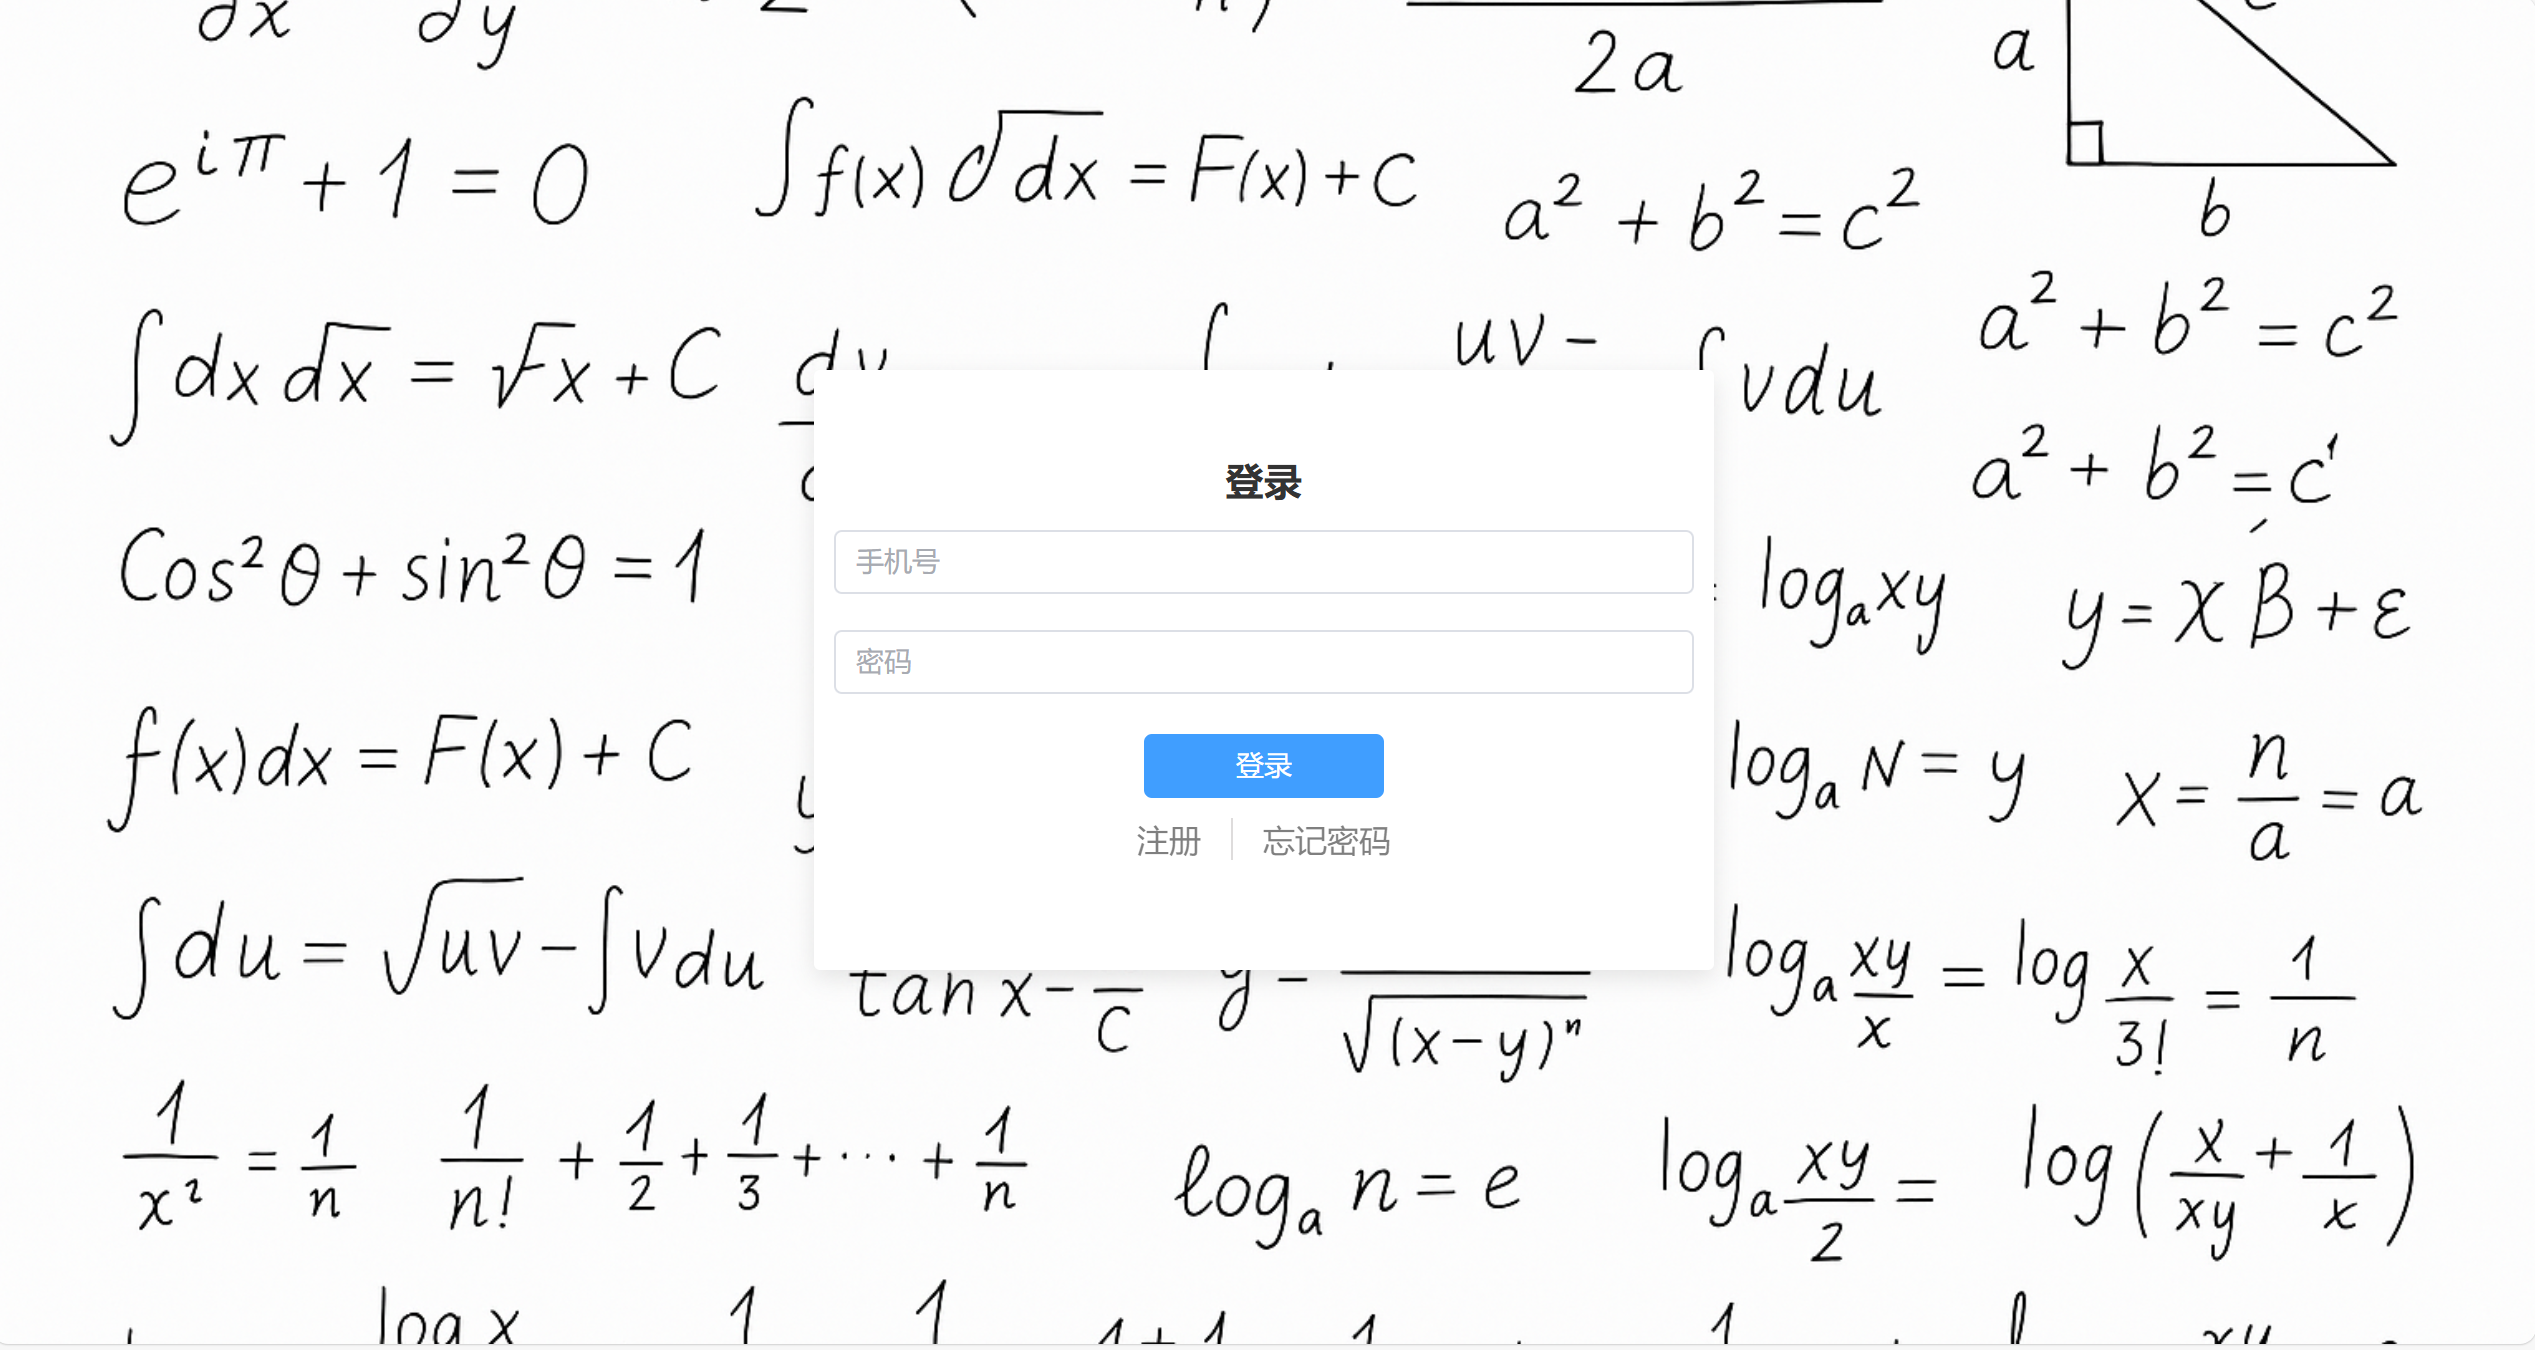
\includegraphics[width=\linewidth]{./图片/登录界面.png}
	\caption{登录界面}\label{登录界面}
\end{figure}

注册界面:

\begin{figure}[H]
	\centering
	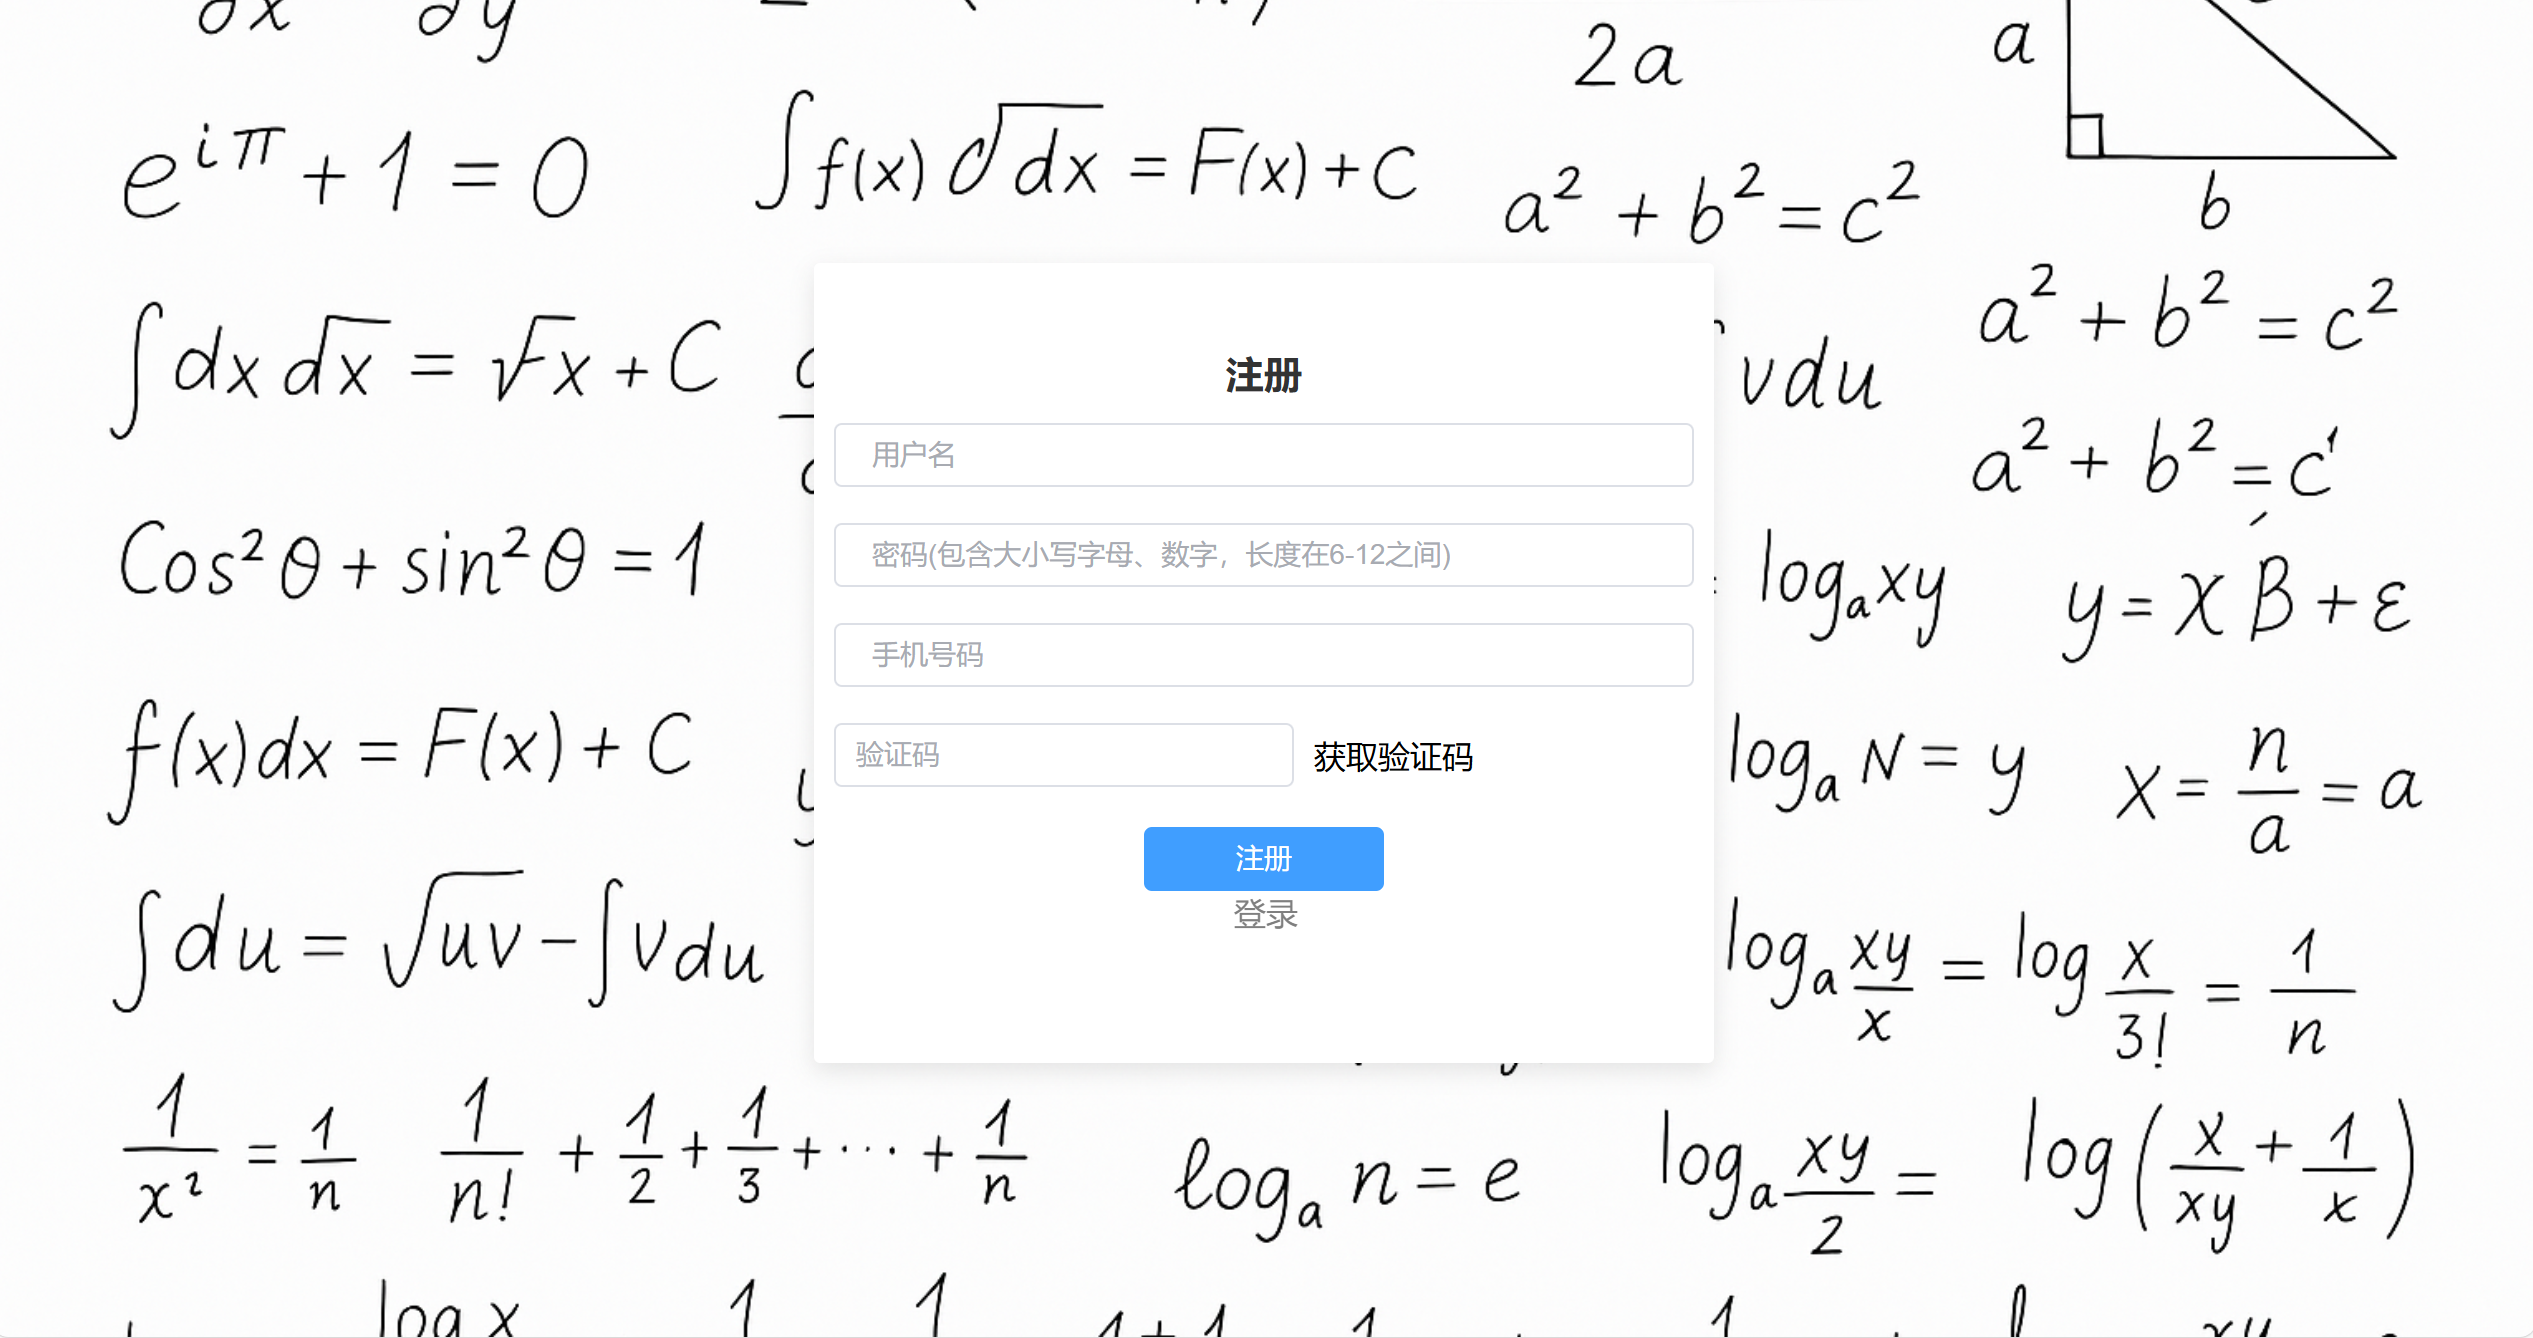
\includegraphics[width=\linewidth]{./图片/注册界面.png}
	\caption{注册界面}\label{注册界面}
\end{figure}

忘记密码界面:

\begin{figure}[H]
	\centering
	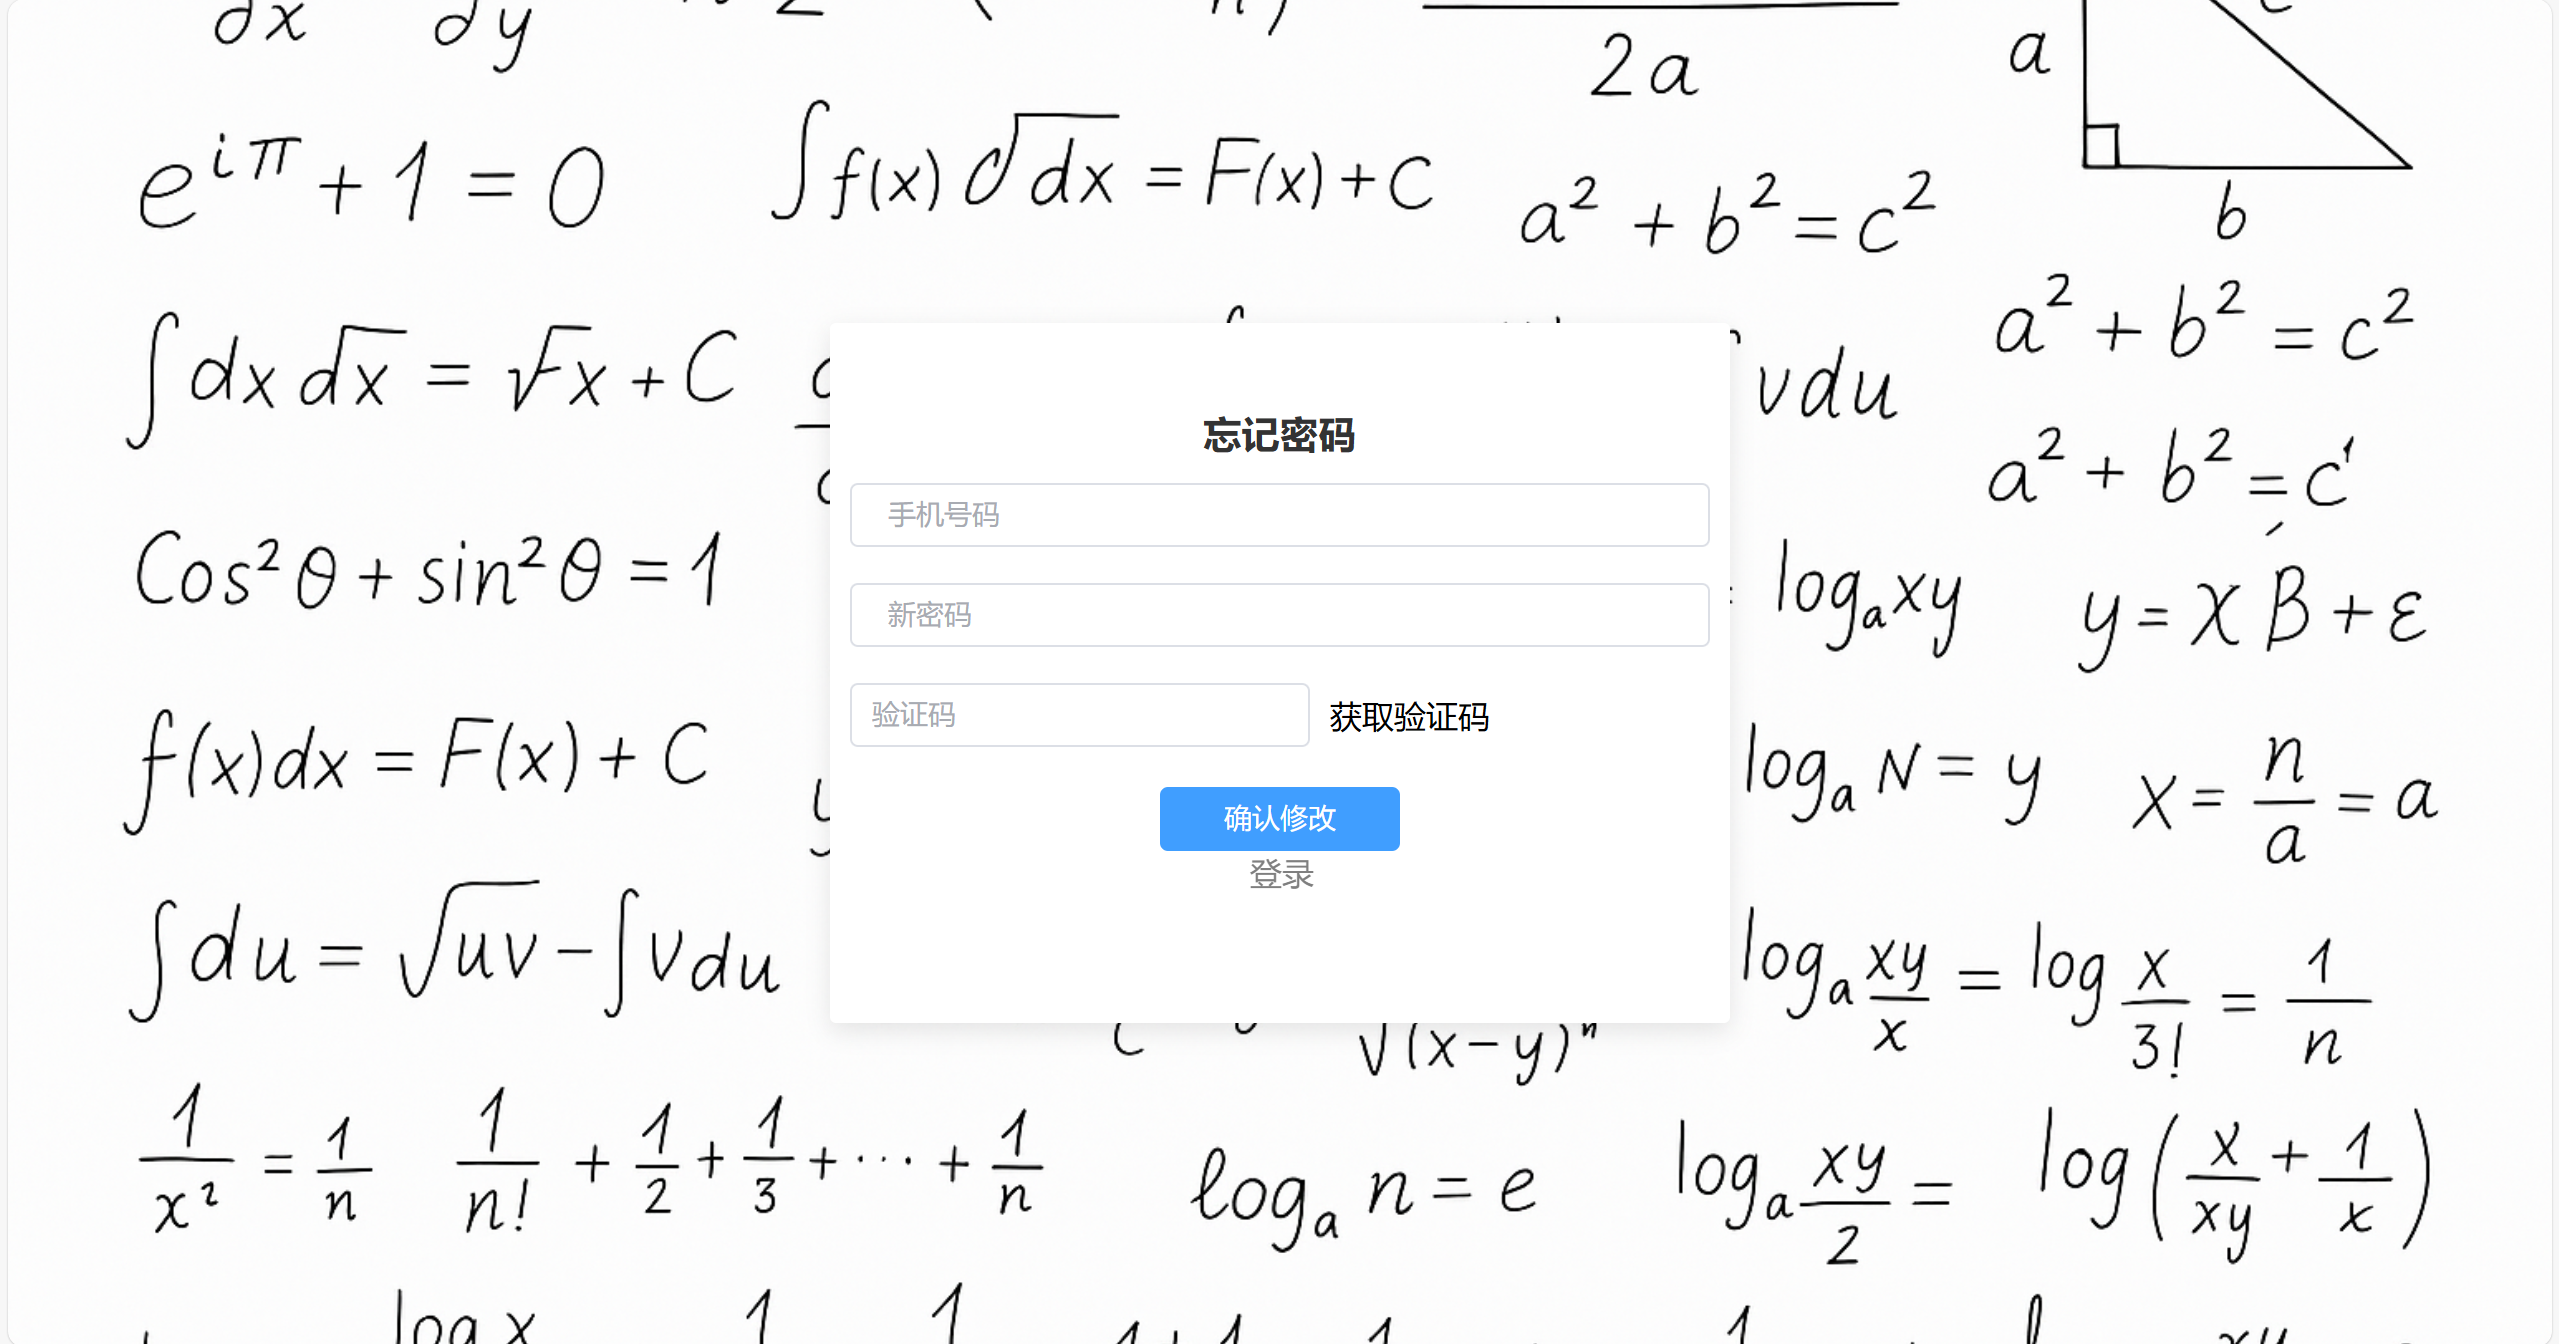
\includegraphics[width=\linewidth]{./图片/忘记密码界面.png}
	\caption{忘记密码界面}\label{忘记密码界面}
\end{figure}

题目列表界面:

\begin{figure}[H]
	\centering
	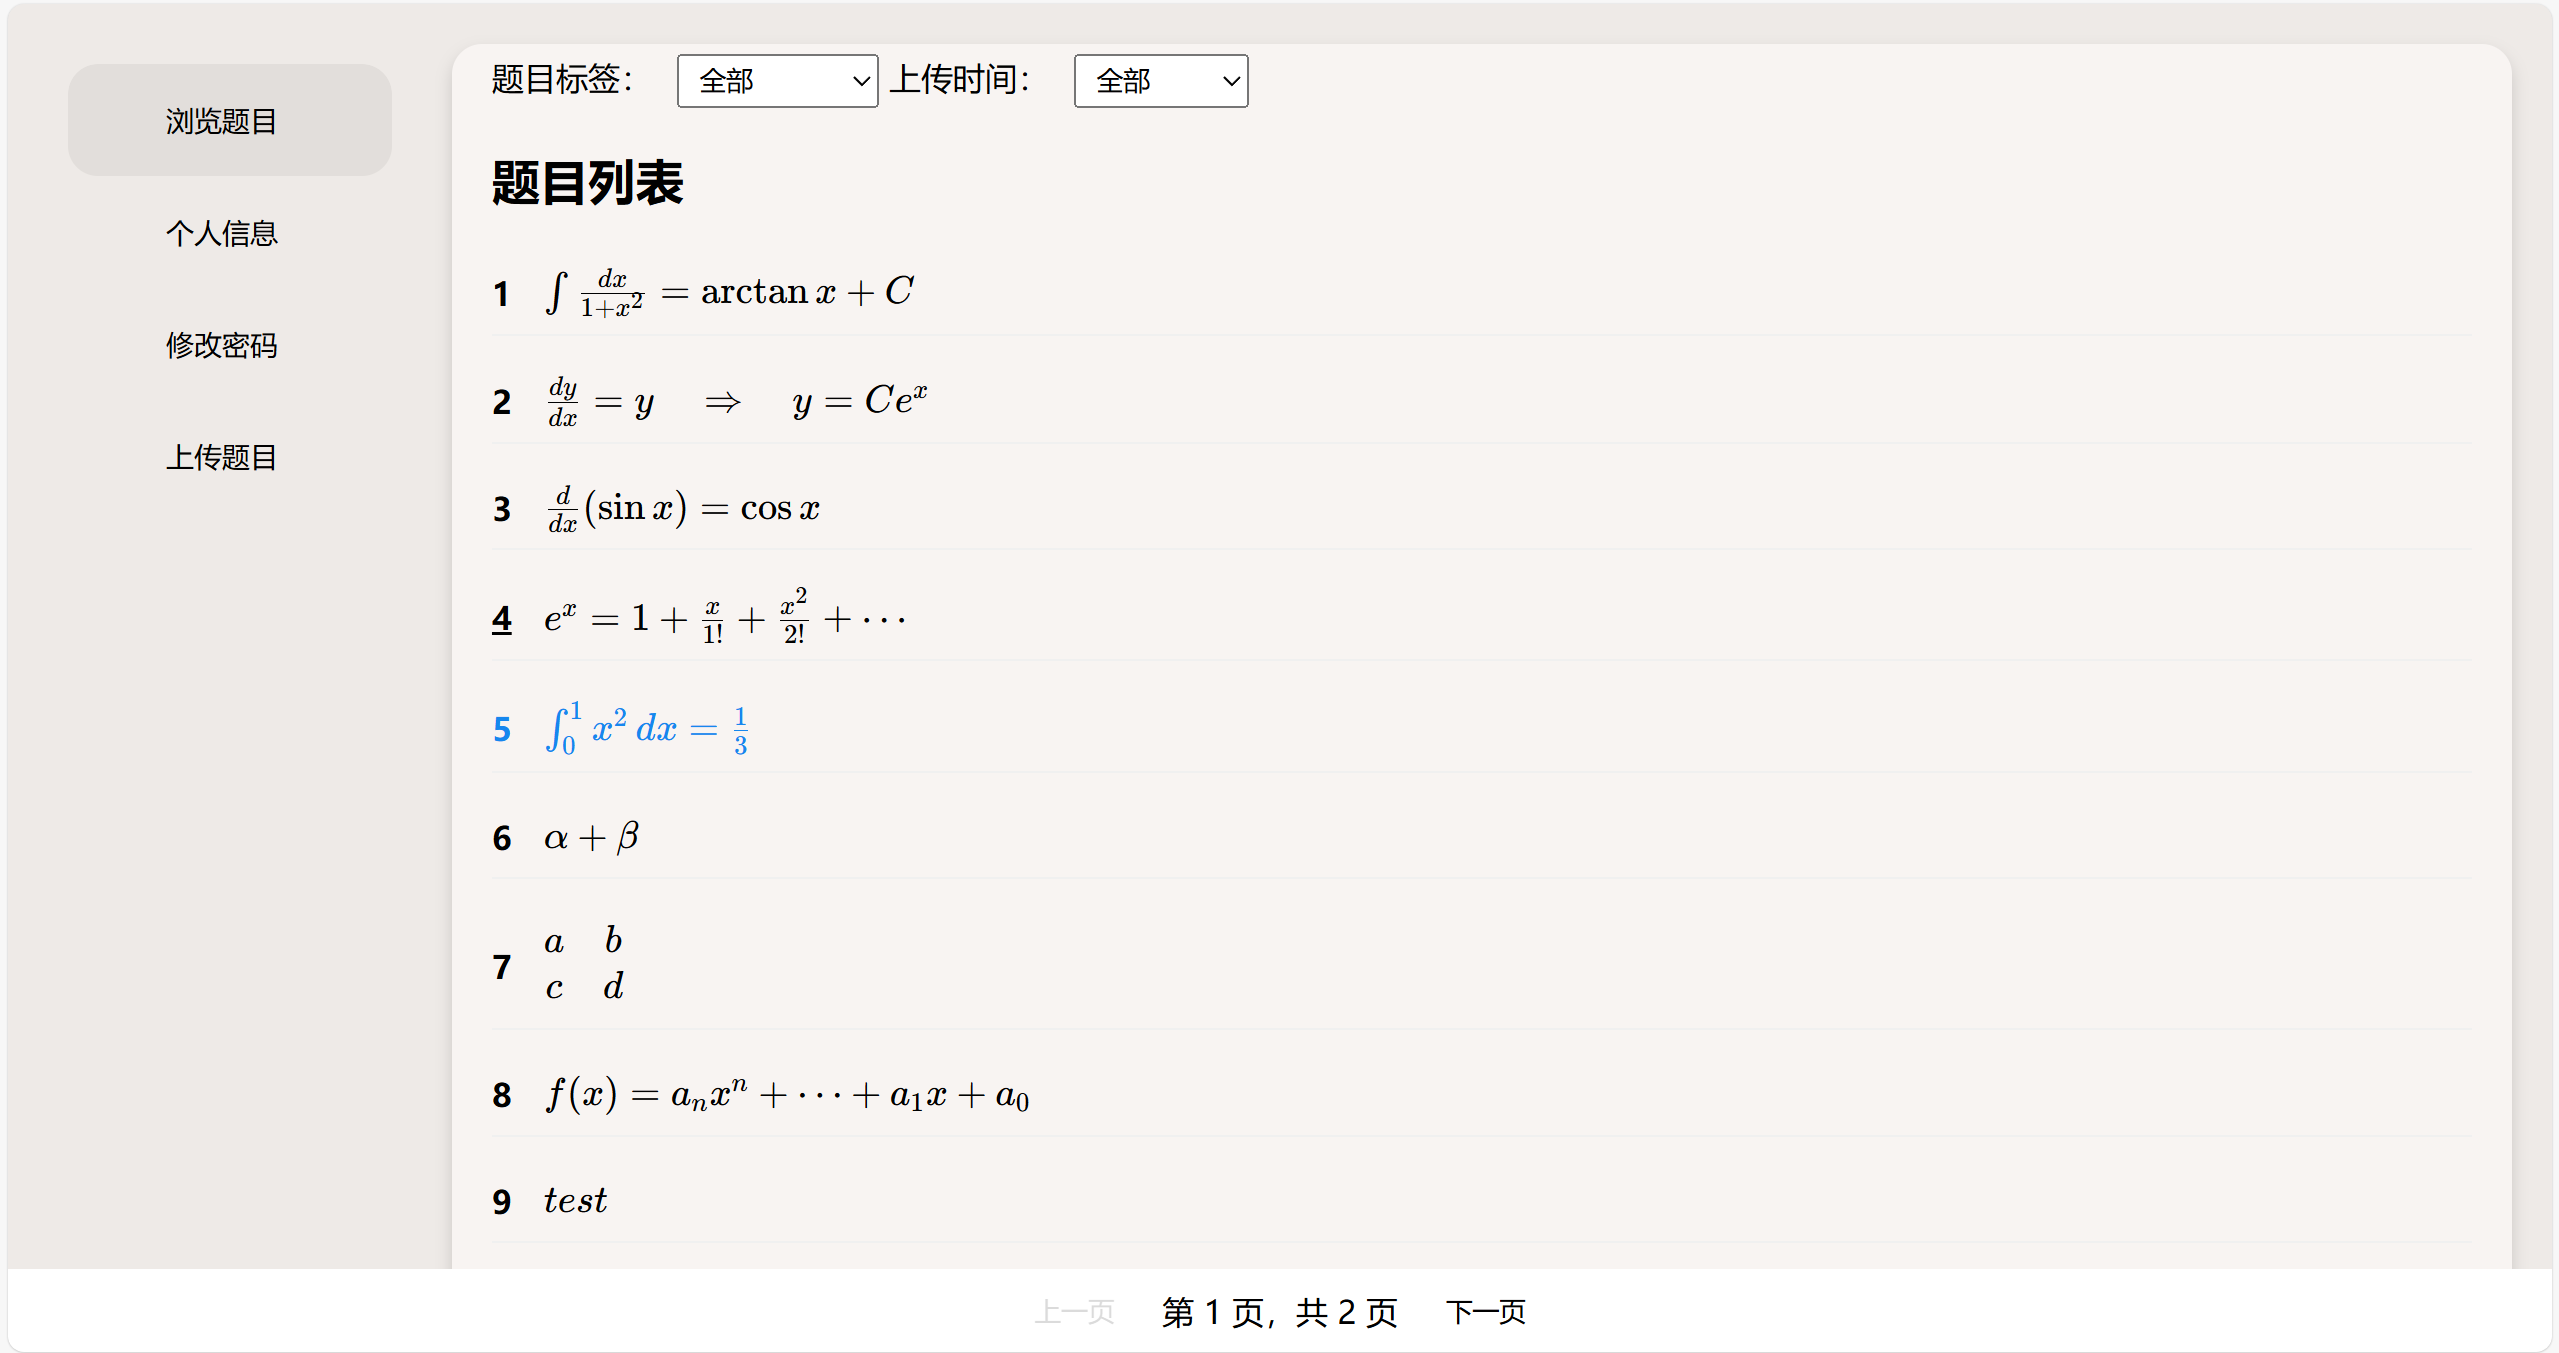
\includegraphics[width=\linewidth]{./图片/题目列表界面.png}
	\caption{题目列表界面}\label{题目列表界面}
\end{figure}

完整题目界面:

\begin{figure}[H]
	\centering
	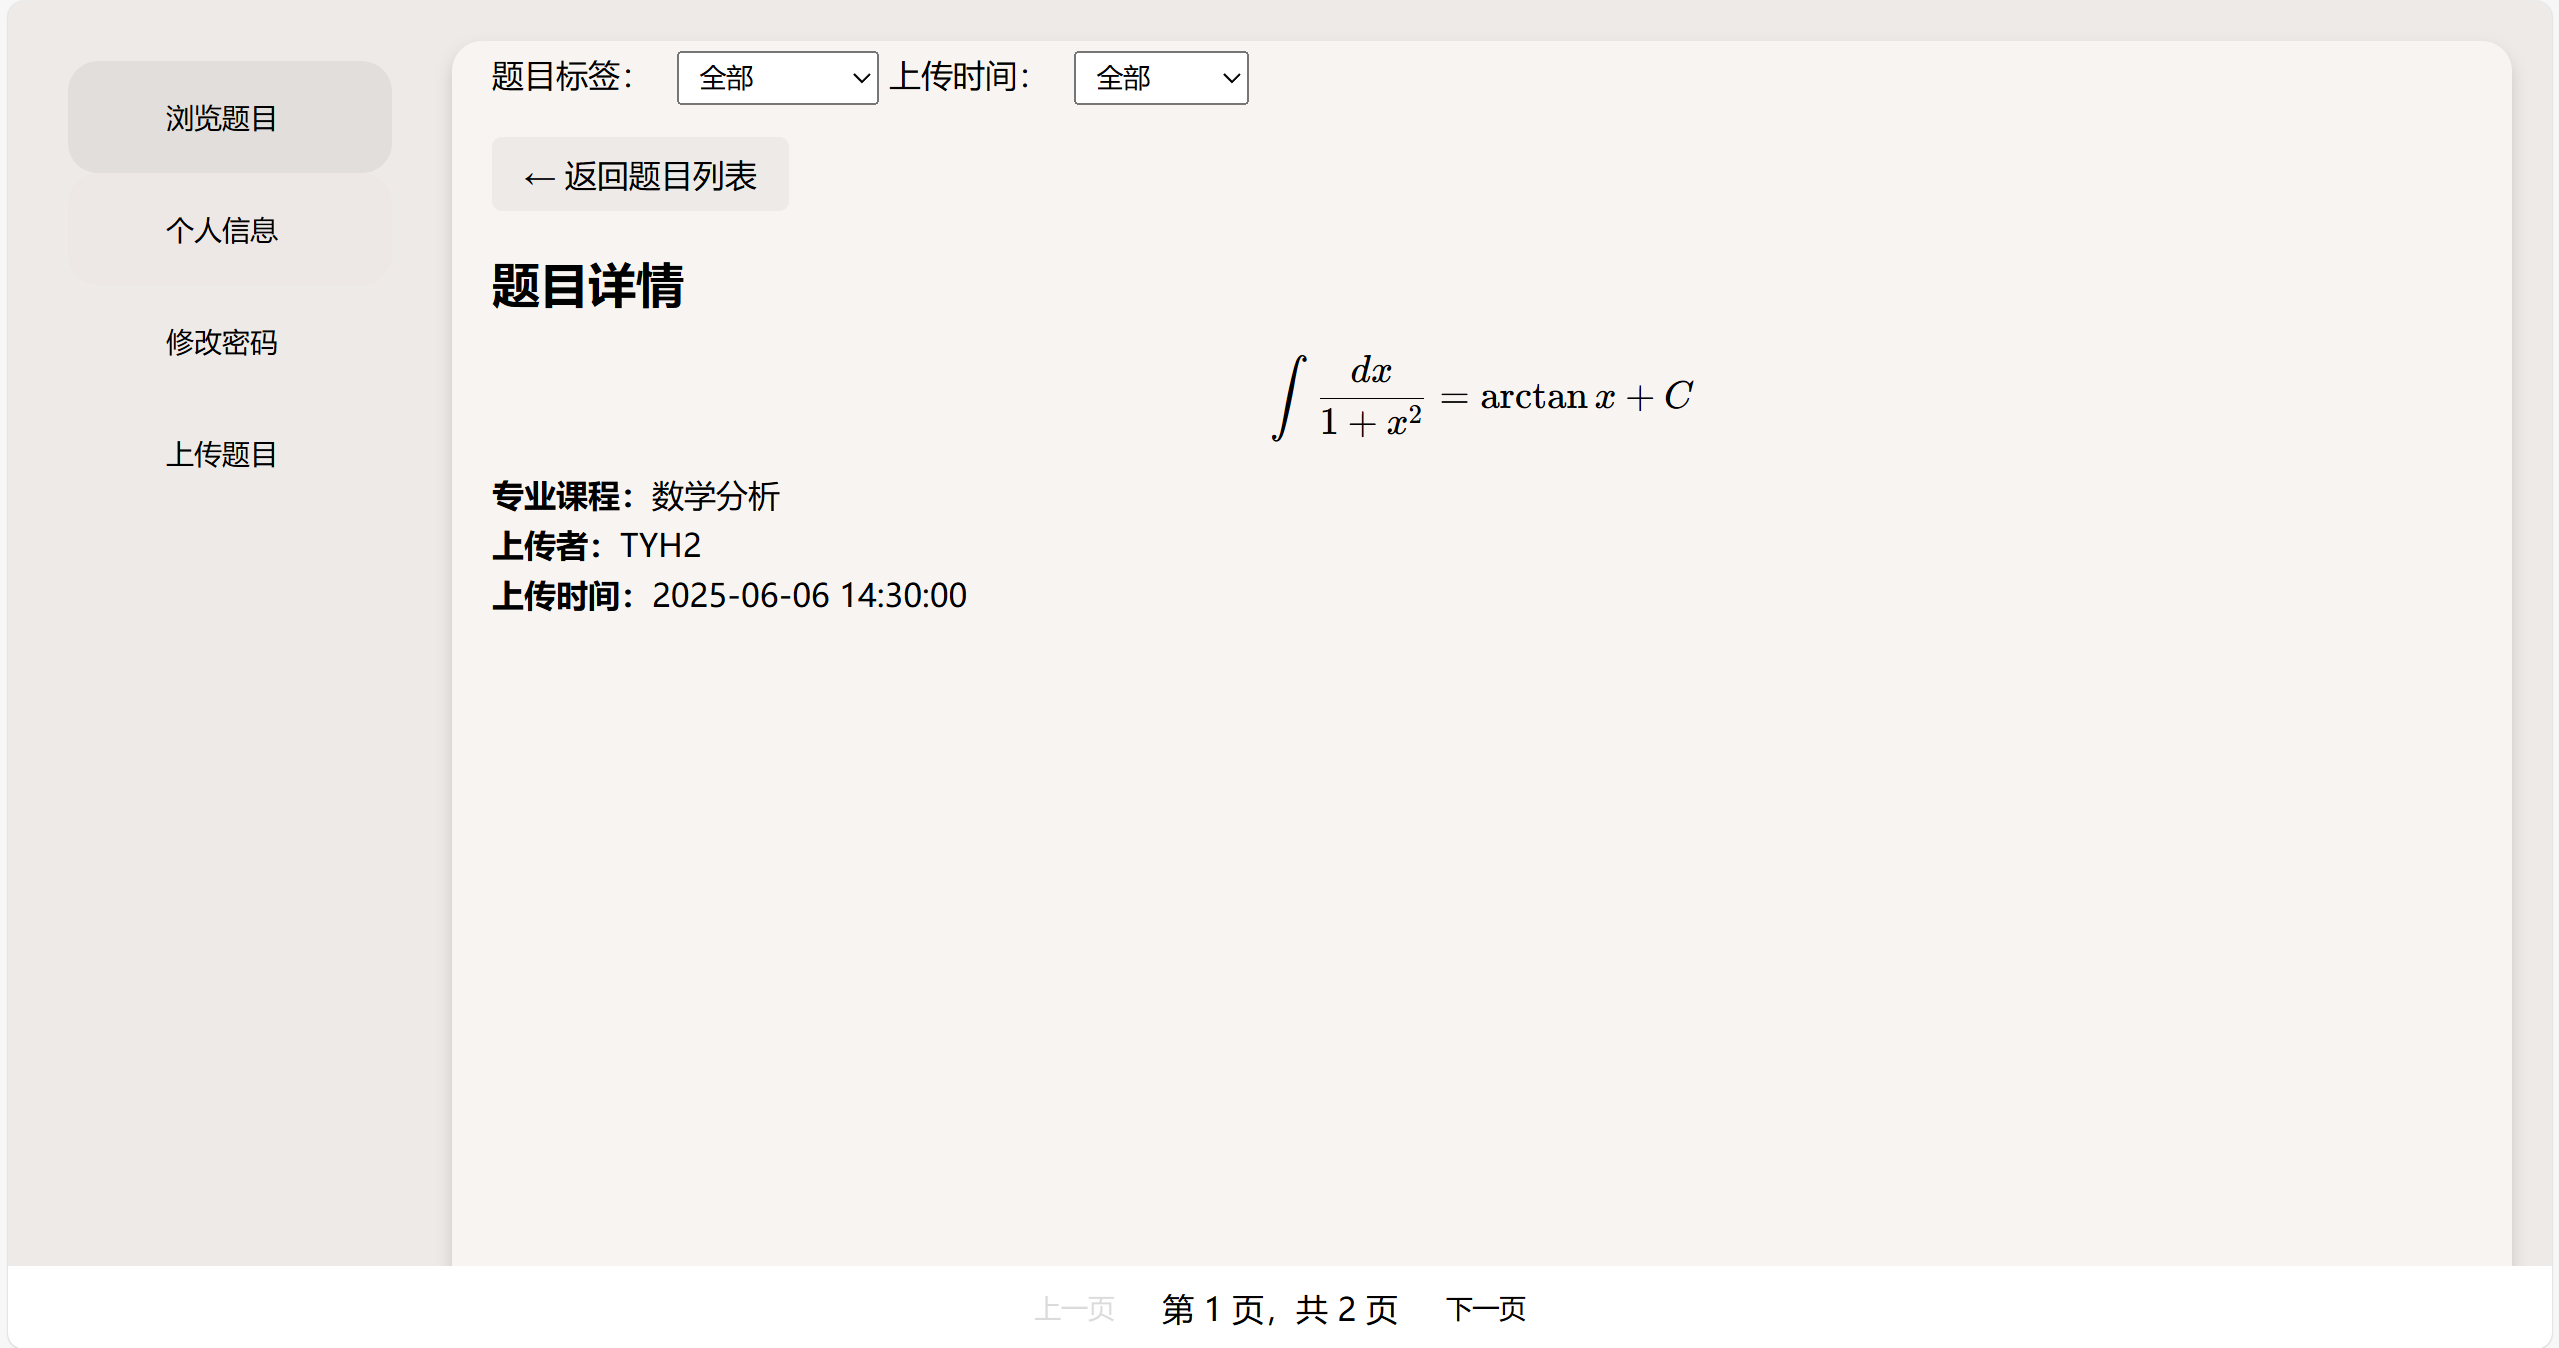
\includegraphics[width=\linewidth]{./图片/完整题目界面.png}
	\caption{完整题目界面}\label{完整题目界面}
\end{figure}

个人信息界面:

\begin{figure}[H]
	\centering
	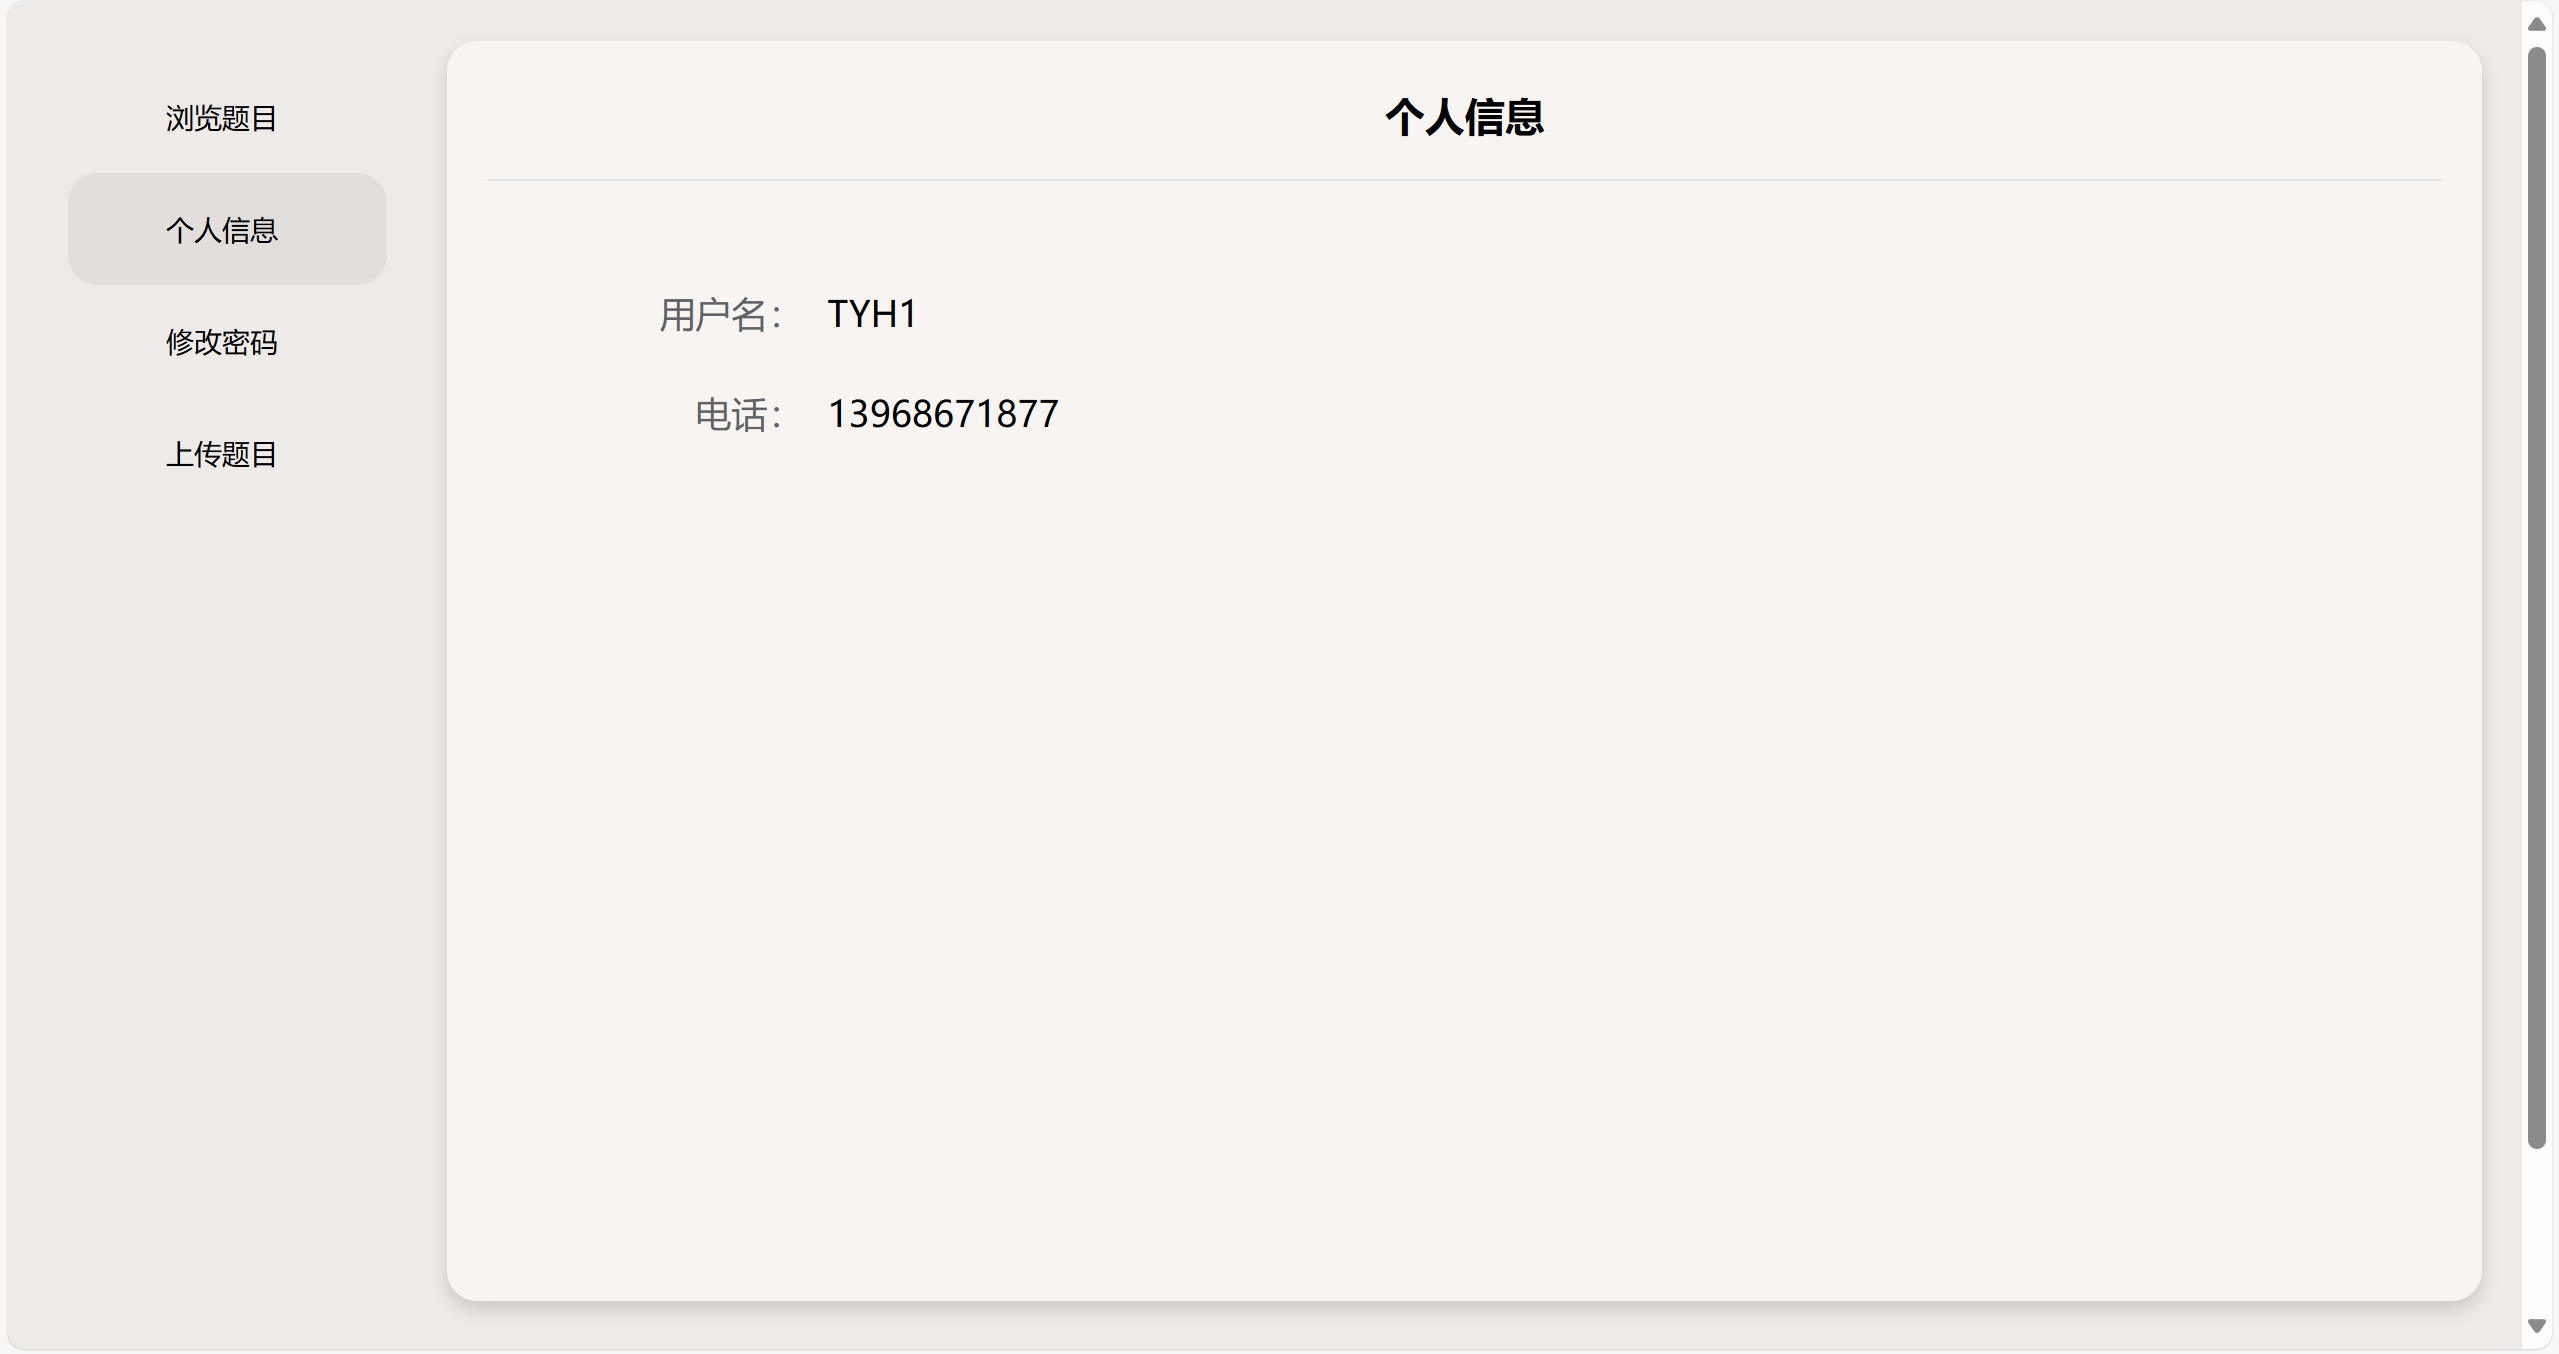
\includegraphics[width=\linewidth]{./图片/个人信息界面.png}
	\caption{个人信息界面}\label{个人信息界面}
\end{figure}

修改密码界面:

\begin{figure}[H]
	\centering
	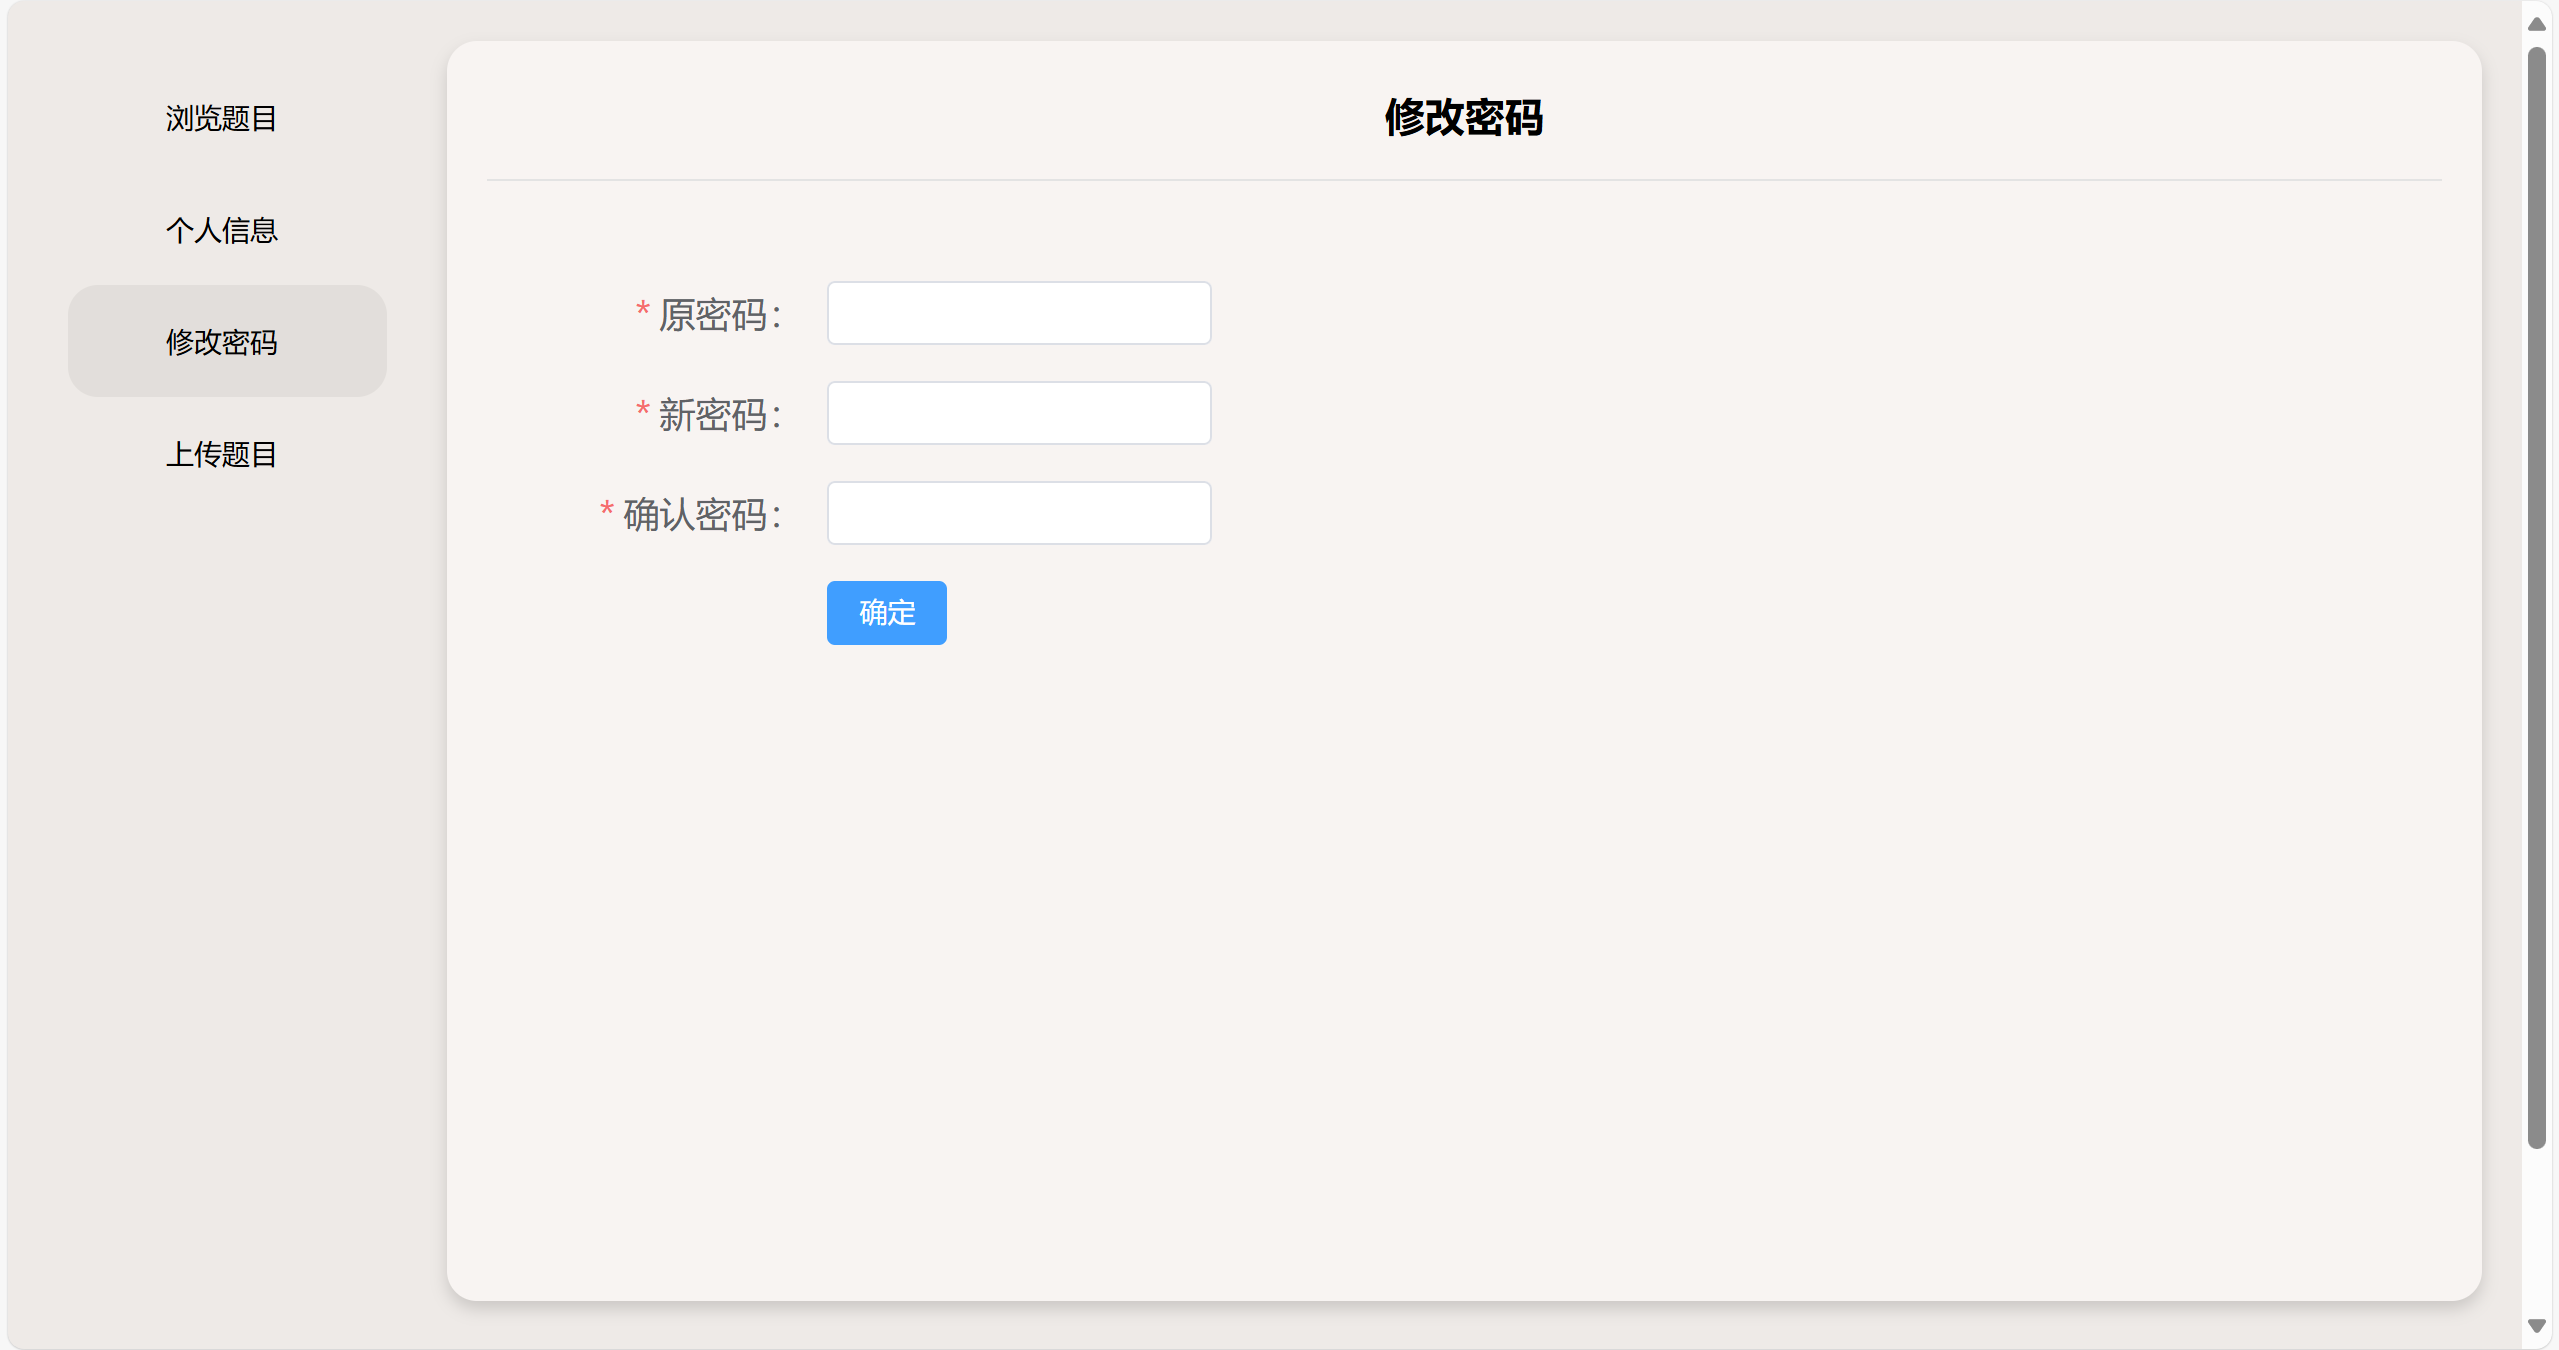
\includegraphics[width=\linewidth]{./图片/修改密码界面.png}
	\caption{修改密码界面}\label{修改密码界面}
\end{figure}

上传题目界面:

\begin{figure}[H]
	\centering
	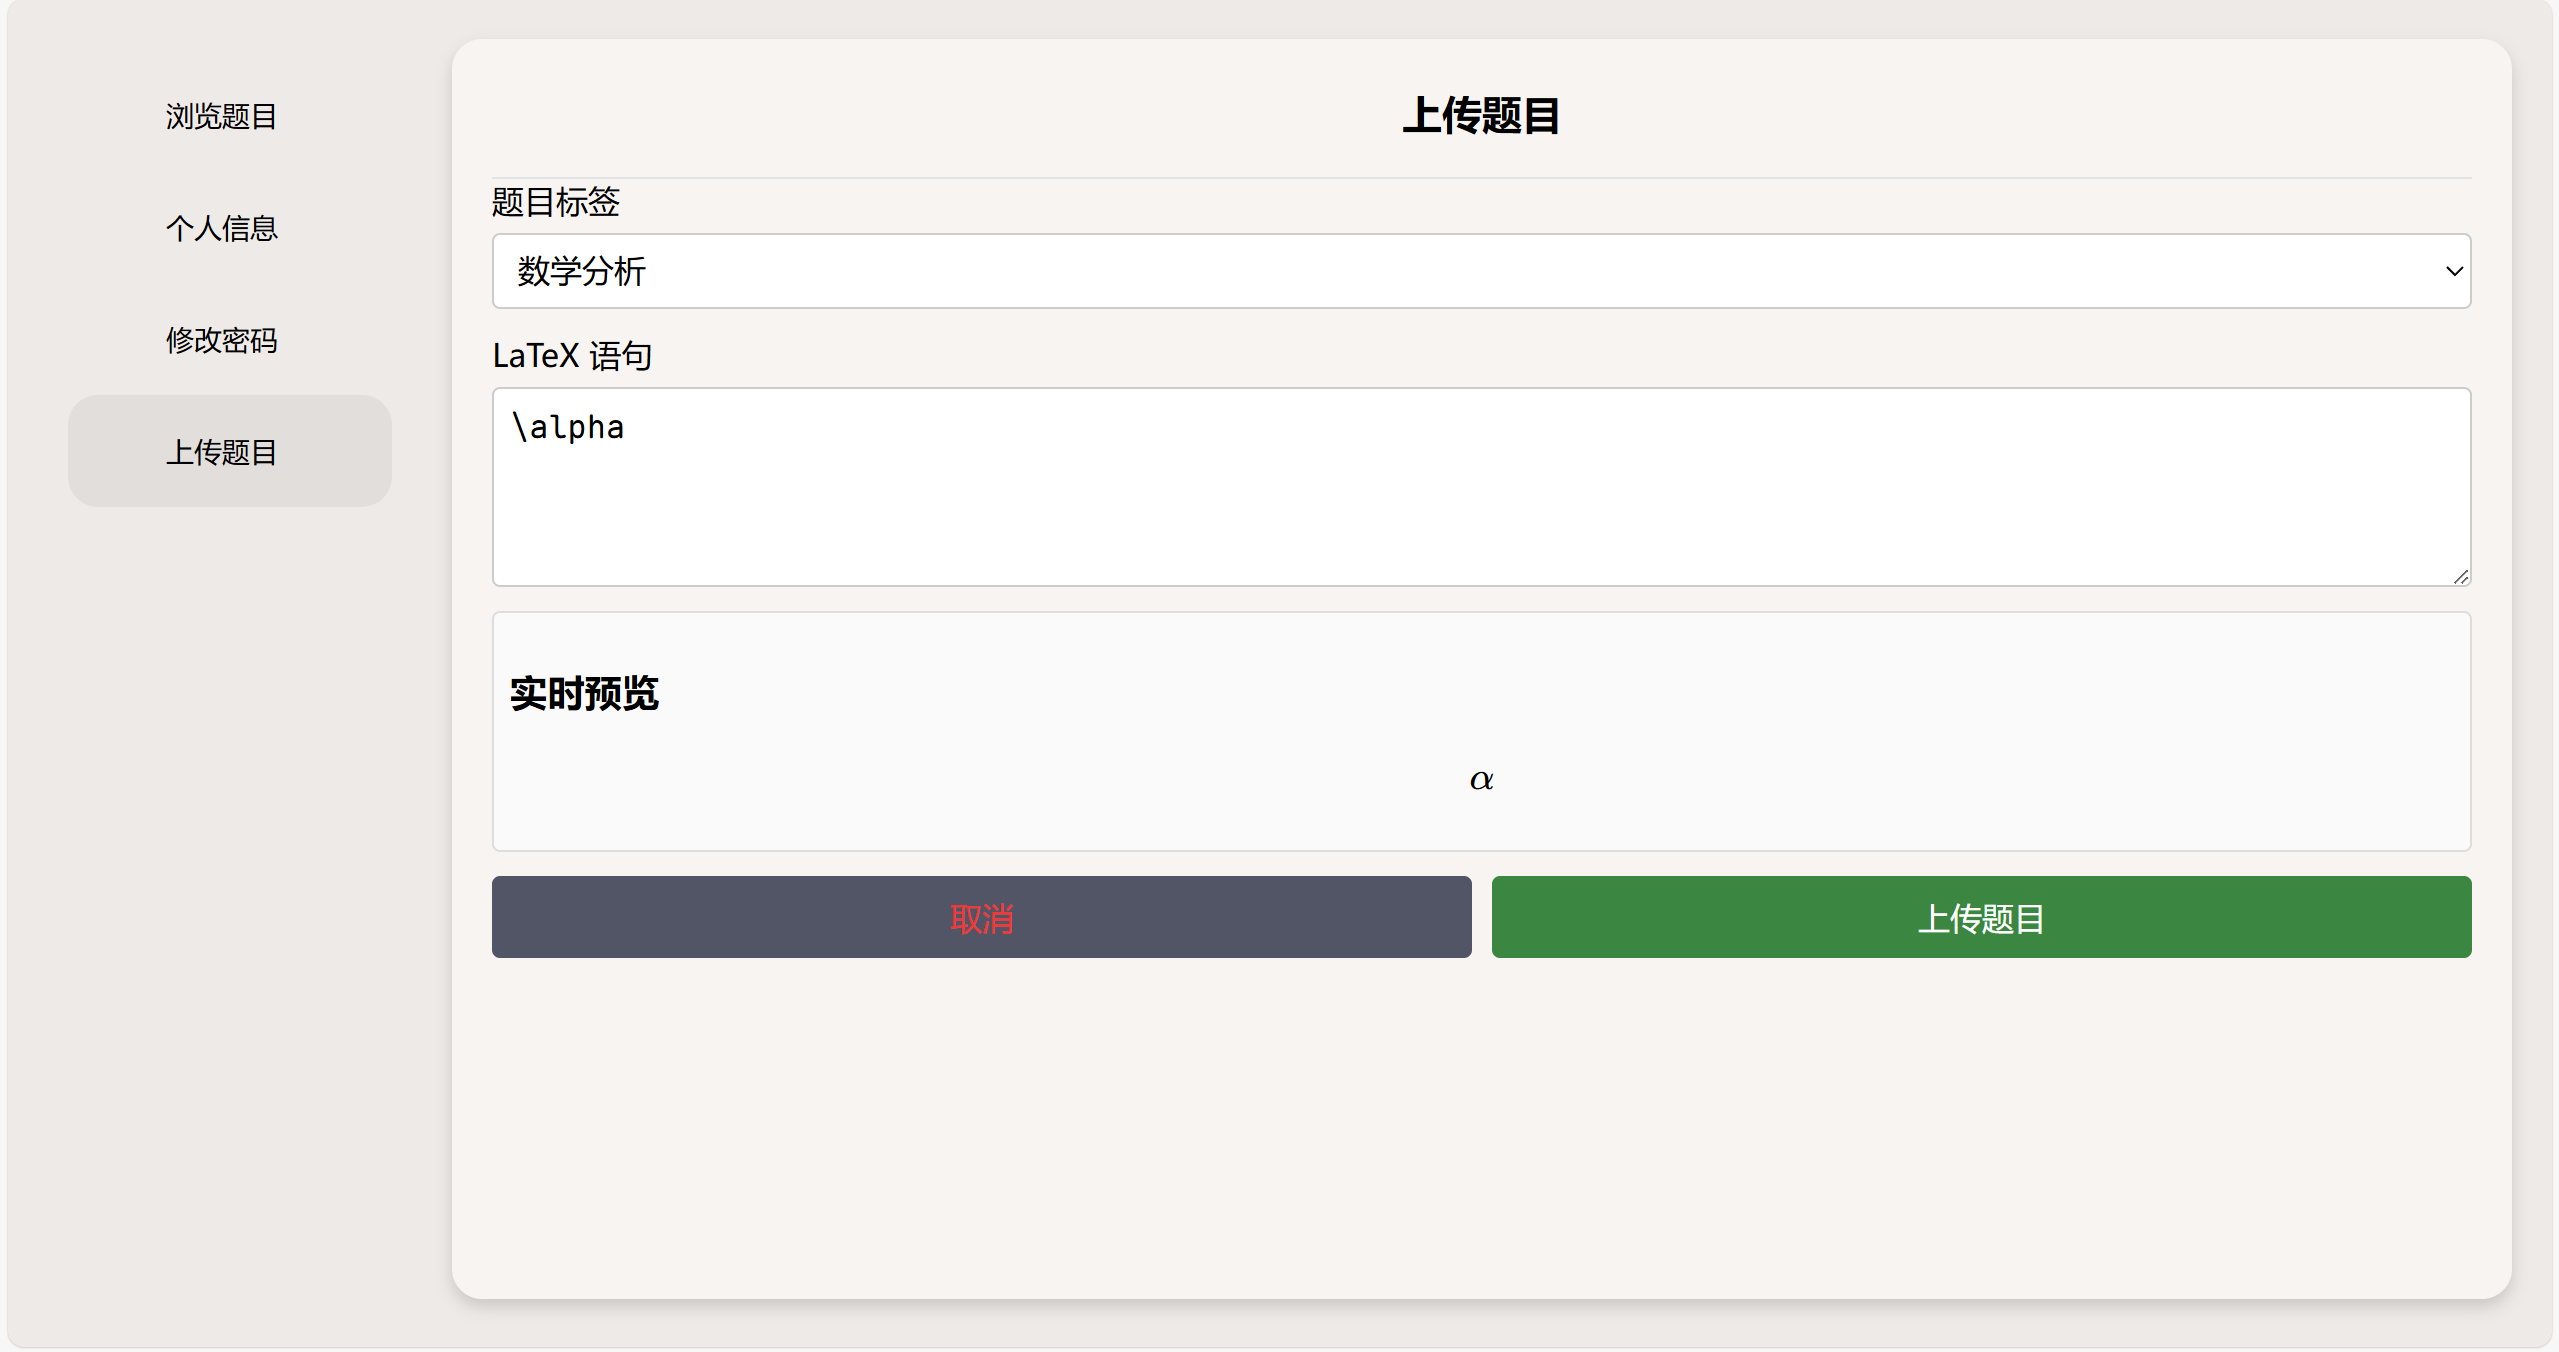
\includegraphics[width=\linewidth]{./图片/上传题目界面.png}
	\caption{上传题目界面}\label{上传题目界面}
\end{figure}

\section*{附录}

SQL脚本:
\begin{lstlisting}
SET NAMES utf8mb4;
SET FOREIGN_KEY_CHECKS = 0;

-- ----------------------------
-- Table structure for problems
-- ----------------------------
DROP TABLE IF EXISTS `problems`;
CREATE TABLE `problems`  (
  `id` int NOT NULL,
  `content` varchar(10000) CHARACTER SET utf8mb4 COLLATE utf8mb4_0900_ai_ci NOT NULL,
  `tag` varchar(20) CHARACTER SET utf8mb4 COLLATE utf8mb4_0900_ai_ci NOT NULL,
  `Uploader` varchar(20) CHARACTER SET utf8mb4 COLLATE utf8mb4_0900_ai_ci NOT NULL,
  `Upload_time` datetime NOT NULL,
  PRIMARY KEY (`id` DESC) USING BTREE
) ENGINE = InnoDB CHARACTER SET = utf8mb4 COLLATE = utf8mb4_0900_ai_ci ROW_FORMAT = Dynamic;

-- ----------------------------
-- Table structure for tags
-- ----------------------------
DROP TABLE IF EXISTS `tags`;
CREATE TABLE `tags`  (
  `id` int NOT NULL,
  `tag_name` varchar(20) CHARACTER SET utf8mb4 COLLATE utf8mb4_0900_ai_ci NULL DEFAULT NULL,
  PRIMARY KEY (`id`) USING BTREE
) ENGINE = InnoDB CHARACTER SET = utf8mb4 COLLATE = utf8mb4_0900_ai_ci ROW_FORMAT = Dynamic;

-- ----------------------------
-- Table structure for user
-- ----------------------------
DROP TABLE IF EXISTS `user`;
CREATE TABLE `user`  (
  `id` int NOT NULL COMMENT '用户id',
  `username` varchar(20) CHARACTER SET utf8mb4 COLLATE utf8mb4_0900_ai_ci NOT NULL COMMENT '用户名',
  `telephone` varchar(20) CHARACTER SET utf8mb4 COLLATE utf8mb4_0900_ai_ci NOT NULL COMMENT '电话号码',
  `password` varchar(255) CHARACTER SET utf8mb4 COLLATE utf8mb4_0900_ai_ci NOT NULL,
  `role` int NOT NULL COMMENT '0表示用户,1表示管理员',
  PRIMARY KEY (`id`) USING BTREE
) ENGINE = InnoDB CHARACTER SET = utf8mb4 COLLATE = utf8mb4_0900_ai_ci ROW_FORMAT = Dynamic;

SET FOREIGN_KEY_CHECKS = 1;
\end{lstlisting}

完整后端代码:

\begin{lstlisting}
from flask import Flask, jsonify, request
from sqlalchemy import text

from config import BaseConfig
from flask_sqlalchemy import SQLAlchemy
import auth
# from aliyunsms.sms_send import send_sms
import datetime
from redis import StrictRedis

# 创建redis对象
redis_store = StrictRedis(host=BaseConfig.REDIS_HOST, port=BaseConfig.REDIS_PORT, decode_responses=True)

# 跨域
from flask_cors import CORS

app = Flask(__name__)
CORS(app, resources={r"/*": {"origins": "*"}})  # 允许所有来源访问

# 添加配置数据库
app.config.from_object(BaseConfig)
# 初始化拓展,app到数据库的ORM映射
db = SQLAlchemy(app)

# 检查数据库连接是否成功
with app.app_context():
    with db.engine.connect() as conn:
        rs = conn.execute(text("select 1"))
        # print(rs.fetchone())

# 定义问题模型,对应数据库中的 problems 表
class Problem(db.Model):
    __tablename__ = 'problems'
    id = db.Column(db.Integer, primary_key=True)
    content = db.Column(db.String, nullable=False)
    tag = db.Column(db.String, nullable=False)
    Uploader = db.Column(db.String, nullable=False)
    Upload_time = db.Column(db.DateTime, nullable=False)


class Tag(db.Model):
    __tablename__ = 'tags'
    id = db.Column(db.Integer, primary_key=True)
    tag_name = db.Column(db.String, nullable=False, unique=True)  # 确保标签唯一

# 获取手机号
def get_token_phone(token):
    data = auth.decode_func(token)
    phone = data['telephone']
    return phone

# 获取用户名
def get_token_username(token):
    data = auth.decode_func(token)
    username = data.get("username")
    if username:
        return username
    # 如果没有 "username" 字段,可以选择返回默认值 "anonymous"
    return "anonymous"

@app.route("/")
def home():
    return jsonify({
        "message": "系统API服务器运行正常",
        "status": 200,
        "available_endpoints": [
            "/user/login (POST)",
            "/user/shop (GET)",
            "/user/addorder (POST)",
            "/manager/shop (GET/POST/DELETE)"
        ]
    })

# 添加一个简单的健康检查路由
@app.route("/health")
def health_check():
    return jsonify({"status": "OK", "timestamp": datetime.datetime.now().isoformat()})


# 用户登录
@app.route("/user/login", methods=["POST"])
def user_login():
    # print(request.json)
    userTelephone = request.json.get("userTelephone").strip()
    password = request.json.get("password").strip()
    sql = text('SELECT * FROM user WHERE telephone = :telephone AND password = :password')
    params = {'telephone': userTelephone, 'password': password}
    data = db.session.execute(sql, params).first()
    # print(data)
    if data is not None:
        user = {'id': data[0], 'username': data[1], 'telephone': data[2], 'password': data[3]}
        # 生成token
        token = auth.encode_func(user)
        # print(token)
        return jsonify({"code": 200, "msg": "登录成功", "token": token, "role": data[4]})
    else:
        return jsonify({"code": 1000, "msg": "用户名或密码错误"})

# 获取用户信息
@app.route("/user/usermsg", methods=["GET"])
def usermsg():
    telephone = get_token_phone(request.headers.get('token'))
    query = text('SELECT username, telephone FROM user WHERE telephone=:telephone')
    result = db.session.execute(query, {'telephone': telephone}).fetchone()

    if result:
            data = dict(username=result.username, telephone=result.telephone)
            return jsonify(status=200, data=data)
    else:
        return jsonify(status=404, message="User not found")


# 更改密码
@app.route("/user/pwd_chg", methods=["POST"])
def user_pwd_chg():
    try:
        data = request.get_json()
        new_pwd = data.get('new_pwd')
        old_pwd = data.get('old_pwd')
        token = request.headers.get('token')
        if not token:
            return jsonify(status=400, msg='缺少 token'), 400

        phone = get_token_phone(token)

        # 参数化查询,避免使用字符串拼接
        query = text('SELECT * FROM user WHERE telephone=:phone AND password=:old_pwd')
        user_data = db.session.execute(query, {"phone": phone, "old_pwd": old_pwd}).fetchall()
        if not user_data:
            return jsonify(status=1000, msg="原始密码错误")
        else:
            update_query = text('UPDATE user SET password=:new_pwd WHERE telephone=:phone')
            db.session.execute(update_query, {"new_pwd": new_pwd, "phone": phone})
            db.session.commit()
            return jsonify(status=200, msg="修改成功")
    except Exception as e:
        db.session.rollback()
        print("Error in user_pwd_chg:", e)
        return jsonify(status=500, msg=str(e)), 500


# 获取题目接口,从数据库中查询 problems 表
@app.route("/api/problems", methods=["GET"])
def get_problems():
    try:
        sql = text("SELECT id, content, tag, Uploader, Upload_time FROM problems")
        result = db.session.execute(sql).fetchall()
        problems = []
        for row in result:
            problems.append({
                'id': row[0],
                'content': row[1],
                'tag': row[2],
                'Uploader': row[3],
                'Upload_time': row[4].strftime('%Y-%m-%d %H:%M:%S') if row[4] else None
            })
        return jsonify({"status": 200, "data": problems})
    except Exception as e:
        return jsonify({"status": 500, "msg": str(e)})


# 上传题目接口(POST 方法),用于写入题目数据到 problems 表中
@app.route("/api/problems", methods=["POST"])
def add_problem():
    data = request.get_json()
    if not data:
        return jsonify({"status": 400, "message": "No input data provided"}), 400

    content = data.get("content")
    tag = data.get("tag", "无标签")
    Uploader = data.get("Uploader", "anonymous")
    Upload_time_str = data.get("Upload_time")

    # 检查必要字段
    if not content:
        return jsonify({"status": 400, "message": "内容不能为空"}), 400
    if not Upload_time_str:
        return jsonify({"status": 400, "message": "Upload_time 不能为空"}), 400

    # 将上传时间字符串转换为 datetime 对象
    try:
        Upload_time = datetime.datetime.fromisoformat(Upload_time_str)
    except Exception as e:
        return jsonify({"status": 400, "message": f"Upload_time 格式错误: {str(e)}"}), 400

    # 查询当前表中的最大 id
    try:
        result = db.session.execute(text("SELECT MAX(id) FROM problems")).fetchone()
        max_id = result[0] if result[0] is not None else 0
    except Exception as e:
        return jsonify({"status": 500, "message": f"查询最大ID失败: {str(e)}"}), 500

    new_id = max_id + 1

    # 通过请求头中的 token 来获取当前登录用户的用户名
    token = request.headers.get("token")
    username = get_token_username(token)  # 保证这里获取的是正确的用户名

    # 创建新的题目记录时,手动指定 id
    new_problem = Problem(
        id=new_id,
        content=content,
        tag=tag,
        Uploader=username,
        Upload_time=Upload_time
    )

    try:
        db.session.add(new_problem)
        db.session.commit()
    except Exception as e:
        db.session.rollback()
        return jsonify({"status": 500, "message": f"写入数据库出错: {str(e)}"}), 500

    return jsonify({
        "status": 200,
        "message": "题目上传成功",
        "id": new_problem.id
    }), 200


# 获取所有标签
@app.route("/api/tags", methods=["GET"])
def get_tags():
    try:
        sql = text("SELECT id, tag_name FROM tags")
        result = db.session.execute(sql).fetchall()
        tag_list = [{"id": row[0], "tag_name": row[1]} for row in result]
        return jsonify({"status": 200, "data": tag_list})
    except Exception as e:
        return jsonify({"status": 500, "msg": str(e)})

if __name__ == '__main__':
    app.run(debug=True, host='127.0.0.1', port=5000)
    # 开启了debug模式
\end{lstlisting}

\end{document}